\documentclass[11pt]{article}
\usepackage[T1]{fontenc}
\usepackage[utf8]{inputenc}
\usepackage{lmodern}
\usepackage{amsmath,amssymb,amsthm,mathtools,bm}
\usepackage[a4paper,margin=27mm]{geometry}
\usepackage{microtype,enumitem,graphicx,booktabs}
\usepackage{xcolor,tikz}
\usetikzlibrary{arrows.meta,calc,decorations.markings,positioning,patterns}
\usepackage[colorlinks=true,linkcolor=blue!45!black,citecolor=blue!45!black,urlcolor=blue!45!black,pdfauthor={OpenAI},pdftitle={The Curve Scaling Limit of Half-Plane Double Dimers}]{hyperref}
\usepackage[capitalise,noabbrev]{cleveref}
\pdfinfoomitdate=1
\pdftrailerid{}
\newtheorem{theorem}{Theorem}[section]
\newtheorem{lemma}[theorem]{Lemma}
\newtheorem{proposition}[theorem]{Proposition}
\newtheorem{corollary}[theorem]{Corollary}
\theoremstyle{definition}
\newtheorem{definition}[theorem]{Definition}
\theoremstyle{remark}
\newtheorem{remark}[theorem]{Remark}
\newcommand{\HH}{\mathbb H}
\newcommand{\DD}{\mathbb D}
\newcommand{\CLE}{\mathrm{CLE}}
\newcommand{\PP}{\mathbb P}
\newcommand{\EE}{\mathbb E}
\newcommand{\1}{\mathbf 1}
\newcommand{\eps}{\varepsilon}
\DeclareMathOperator{\diam}{diam}
\DeclareMathOperator{\dist}{dist}
\DeclareMathOperator{\tr}{tr}
\DeclareMathOperator{\arsinh}{arsinh}
\setlist{topsep=4pt,itemsep=3pt,parsep=0pt}
\setlength{\emergencystretch}{2em}
\allowdisplaybreaks[1]
\title{The Curve Scaling Limit\\of Half-Plane Double Dimers}
\author{OpenAI}
\date{September 23, 2026}
\begin{document}
\maketitle
\begin{abstract}
We prove that the complete double-dimer loop ensemble for the Temperleyan
square lattice in the upper half-plane converges to nested \(\CLE_4\).
The convergence holds along the full mesh limit and matches every macroscopic
loop as an unparametrized curve. This resolves the half-plane Temperleyan form
of the double-dimer \(\CLE_4\) scaling-limit conjecture.
\end{abstract}

\section{Introduction}\label{sec:introduction}

Superposing two independent dimer coverings produces loops whose large-scale
geometry is expected to be conformally invariant. For the square lattice, the
predicted limit is the conformal loop ensemble with parameter \(4\). The
distinction between geometric and topological convergence is important here:
knowing which punctures a loop surrounds does not control thin excursions,
invisible retraced pieces, or repeated traversal of a limiting trace.
We prove the curve convergence for the standard Temperleyan law in the upper
half-plane, retaining every nested generation.

\subsection{The law and the topology}
Write
\[
 \HH=\{z\in\mathbb C:\operatorname{Im}z>0\},\qquad
 \HH_\delta=\HH\cap\delta\mathbb Z^2 .
\]
Edges join nearest neighbors. A dimer covering is a perfect matching.
To specify its infinite-volume law, start with a simple lattice polygon in
the coarse grid \((0,\delta)+2\delta\mathbb Z^2\), retain the fine-grid
vertices and edges in its closure, and delete one coarse boundary vertex,
called the root. Uniform matchings on these finite Temperleyan graphs
converge locally as the polygons exhaust \(\HH\) and their roots escape to
infinity. We use this standard law, equivalently specified by the inverse
Kasteleyn operator vanishing at infinity \cite[Section~2]{BI}.
The coarse-grid translate puts the lower boundary on the bottom row of
\(\HH_\delta\).

Take two independent matchings with this law. Almost surely their
superposition consists of doubled edges and finite simple even cycles
\cite[opening of Section~2]{BI}; see also \cite[Section~5.4, Lemma~26]{Dubedat}.
Delete the doubled edges and let
\(\mathcal L_\delta\) be the collection of all cycles, drawn with straight
edges and regarded as unrooted, unoriented loops.
Nested \(\CLE_4\) means an ordinary nonnested \(\CLE_4\), followed recursively
by conditionally independent copies inside every loop. The normalization is
the one in which the outermost ensemble comes from a Brownian loop soup of
central charge \(1\) \cite{SW}.

Let \(\DD=\{w\in\mathbb C:|w|<1\}\). We fix, throughout, the compactification
\[
 F:\HH\longrightarrow\DD,\qquad F(z)=\frac{z-i}{z+i}.
\]
For continuous loops \(\gamma,\widetilde\gamma:S^1\to\overline{\DD}\), put
\[
 d_{\rm loop}(\gamma,\widetilde\gamma)
 =\inf_{\phi}\sup_{t\in S^1}
       |\gamma(t)-\widetilde\gamma(\phi(t))|,
\]
where \(\phi\) ranges over circle homeomorphisms of either orientation.
We identify loops at zero distance; in particular a weakly monotone change
of parameter, with pauses, does not change the loop.
Collections omit constant loops and have finitely many members of diameter
greater than any fixed positive number, with multiplicities retained.
An \(\eps\)-matching of two
collections is a partial bijection covering every loop of diameter greater
than \(\eps\) on either side, with matched loops at distance at most
\(\eps\). The unmatched loops therefore all have diameter at most
\(\eps\). Convergence means that such matchings exist with
\(\eps\downarrow0\). All diameters and loop distances in this definition
are measured after applying \(F\).

It is convenient to use a compatible metric \(\rho\) on collections.
For a partial bijection, charge the distance of each matched pair and
half the diameter of each unmatched loop; take the supremum of these
charges, then the infimum over partial bijections.
This defines \(\rho\), with the supremum of an empty family equal to zero.
The triangle inequality follows by composing partial bijections: a loop
whose partner becomes unmatched has half-diameter at most the sum of
the two charges, since
\[
 |\diam\gamma-\diam\widetilde\gamma|
       \le 2d_{\rm loop}(\gamma,\widetilde\gamma).
\]
Vanishing \(\rho\) identifies equal collections because there are only
finitely many loops above each positive diameter. A matching of cost at
most \(\eps\) leaves only loops of diameter at most \(2\eps\) unmatched,
so \(\rho\) induces exactly the topology specified above.
We use the inherited topology on the subspace of collections whose loops
are contained in the open disk. This is the target space for the theorem.
The larger closed-disk space will be useful during the compactness proof,
before boundary contact has been excluded.

\begin{theorem}\label{thm:main}
For the half-plane Temperleyan law specified above, the family
\(F(\mathcal L_\delta)\) is tight as \(\delta\downarrow0\) in the
loop-collection topology just defined, and
\[
 F(\mathcal L_\delta)\ \Longrightarrow\ F(\mathcal L),
 \qquad \delta\downarrow0,
\]
where \(\mathcal L\) is standard nested \(\CLE_4\) in \(\HH\).
The convergence holds along the full mesh limit and matches all
macroscopic loops as curves.
\end{theorem}

\subsection{History and the remaining geometric question}
Theorem~\ref{thm:main} resolves the half-plane Temperleyan form of the
double-dimer \(\CLE_4\) scaling-limit conjecture. Two strands of earlier
work explain both its prediction and the remaining obstacle.

Exact dimer enumeration on the square lattice was developed by
Kasteleyn~\cite{Kasteleyn} and Temperley and Fisher~\cite{TemperleyFisher},
using Pfaffian and determinant methods. Lieb~\cite{Lieb} introduced the
transfer-matrix approach. These finite algebraic descriptions provide
the background for our rectangle calculation. At the continuum scale,
Kenyon~\cite{KenyonGFF} proved convergence of appropriately normalized
dimer-height fluctuations for suitable Temperleyan approximations of
smooth Jordan domains to the Gaussian free
field. That field limit motivates the connection with \(\CLE_4\), but
does not by itself give convergence of loop curves: passing from a
distribution-valued field to its interfaces requires additional control.

Further evidence for the interface prediction came from Kenyon and
Wilson~\cite{KW}. For alternating black and white
boundary nodes in the half-plane, they showed that the limiting
double-dimer pairing probabilities agree with those for the corresponding
Gaussian-free-field contour lines. This identifies the
boundary pairings, while leaving convergence of the paths open.
Kenyon~\cite{Kenyon} used quaternionic weights to construct loop-homotopy
observables with conformally invariant scaling limits. Dub\'edat~\cite{Dubedat} identified
a class of these topological correlators with their nested \(\CLE_4\)
counterparts through isomonodromic tau-functions.
Basok and Chelkak~\cite[Corollary~1.7]{BC} recovered probabilities of cylindrical events
from their lamination expansion, subject to a continuum lamination-tail
estimate; Bai and Wan~\cite[Corollary~1.5]{BW} supplied that estimate
for the nested ensemble.
We use the precise half-plane formulation in Basok and Izyurov's
preprint~\cite[Theorem~4.2(2), Eq.~(4.17)]{BI}.
It retains all nested generations. Basok and Izyurov also prove local
Gaussian fluctuations and convergence of the centered nesting field,
which describe further aspects of the ensemble beyond a fixed puncture
record.

The distinction needed here is between those puncture records and
convergence in the curve topology. A long thin excursion may surround
none of the selected points. Moreover, even equality of a limiting trace
and winding number one allows a path to move backward along an arc before
continuing forward. We must control both effects while retaining the
number of loops and their nesting. The new estimates address these
geometric questions directly.

\subsection{The geometric estimates and the proof}

The new input consists of two geometric estimates in a corner-rooted
Temperleyan rectangle. The first bounds the total number of disjoint
traversals of a fixed-width slab, including multiple traversals by a single
loop. It supplies both macroscopic loop counts and moduli of continuity
after reparametrization. The second controls the signed crossing counts
of arcs whose endpoints reach prescribed opposite sides of the slab;
the sign records the direction of a crossing. On a shrinking transverse
interval it excludes an arc's nonzero count disagreeing with that of its
whole loop, and simultaneous nonzero counts from arcs on distinct loops.
After localization, this prevents cancellation of an excursion against a
return path that finite-puncture data would fail to see.

Both estimates come from a transfer matrix counting dimer configurations
column by column. A boundary state records which dimers cross the seam
between columns. Complementing alternate occupancy bits turns such a
state into a subset of transverse sites, called a particle state; the
column transfer is an exterior power of a one-particle matrix.
This uses Lieb's transfer method~\cite{Lieb}, with sine modes and
particle sectors corresponding to the open-boundary spectral analysis of
Rasmussen and Ruelle~\cite[Section~IV~A]{RR}. We derive the needed formulas in
the convention appropriate to the deleted corner and prove the cap
normalization explicitly, where a cap is the part of the rectangle on
one side of a chosen seam.
Changing particle number by a large amount gives a quadratic spectral
penalty and hence traversal tightness. A two-particle insertion supported
on a short interval moves two occupied sites from one matching's state to
the other's. Its matrix coefficients are two-by-two minors
of an interval projection. Modes spread across the transverse sites make these coefficients
quadratic in the interval length. To turn that signed insertion into a
probability bound, we prove a pointwise positivity identity, weighting
nested loop portions cut off by transverse lines, so that contributions
decrease geometrically down each
nesting chain. This separation of a local operator estimate from a planar
positivity argument is the main technical mechanism. The estimates are
proved in Sections~\ref{sec:transfer} and~\ref{sec:short-segment}.

Wilson's algorithm and the Temperley correspondence~\cite{Wilson,PW,KPW}
transfer the estimates
to bounded half-plane windows, uniformly in the mesh
(Section~\ref{sec:localization}). That section then proves compactness by
constructing parametrizations directly from the fixed-slab estimates.
The passage from crossing counts to controlled parametrizations follows
the method of Aizenman and Burchard~\cite[Lemma~2.4 and Section~4]{AB}.

Section~\ref{sec:identification} couples a subsequential path limit and
its puncture records with a canonical nested \(\CLE_4\). It fixes each
finite puncture grid before choosing a sufficiently small lattice mesh.
On the resulting joint realization, a pathwise argument rules out
invisible curves and identifies each visible trace. A second grid
refinement then excludes backtracking along that trace. This last step
recovers the traversal order that trace equality and winding number one
leave undetermined.

\subsection{Established inputs}\label{sec:inputs}
We state precisely the information imported from the literature. A
lamination relative to a finite set of punctures records the homotopy
classes of disjoint simple loops in the punctured domain, including their
multiplicities. Delete every loop surrounding at most one puncture.
The remaining record will be called the reduced lamination.

\begin{theorem}[Cylindrical convergence {\cite[Theorem~4.2(2)]{BI}}]
\label{thm:cylindrical}
Let \(z_1,\ldots,z_r\) be distinct interior points of \(\HH\), and choose
face punctures \(z_j^\delta\to z_j\). For the two independent matchings
used in Theorem~\ref{thm:main}, the reduced lamination relative to
\((z_j^\delta)_{j=1}^r\) converges in law to the corresponding reduced
lamination of nested \(\CLE_4\). In particular the multisets of enclosed
puncture subsets, with multiplicities and with subsets of size at most
one deleted, converge in law.
\end{theorem}

The precise input is equation~(4.17) of the cited theorem in the
January~2, 2025 preprint version. It is uniform when the puncture tuples remain in a compact
set away from collisions. We only need the weaker formulation above.
For a fixed puncture set the lamination state space is countable.
Convergence of its point probabilities to a probability law implies total
variation convergence: first restrict to a finite set carrying nearly all
limiting mass. Passing to enclosed subsets is then a measurable
pushforward; we do not claim that subsets determine every homotopy class.
Later refinements always fix a finite puncture configuration before taking
the lattice mesh sufficiently small.

\begin{proposition}[Standard properties of nested \(\CLE_4\)]
\label{prop:cle-facts}
After conformal transport to the disk, nested \(\CLE_4\) consists almost
surely of pairwise disjoint simple loops contained in the open disk.
There are finitely many loops of diameter greater than any positive
number. Every fixed interior point is almost surely off all loop traces
and is surrounded by infinitely many successive nested loops.
\end{proposition}

The nonnested properties and the recursive construction are established in
\cite[Sections~2.1--2.2]{SW}. In particular, every fixed interior point is
surrounded almost surely; conditional iteration in the successive loop
interiors gives infinitely many surrounding loops and avoidance of all
traces. Children lie strictly inside their parents, so disjointness also
persists across generations. Bounded-domain macroscopic finiteness for the
entire nested ensemble is recorded explicitly in \cite[p.~2788]{BC}.
We also use the classical Temperley correspondence \cite[Theorem~1]{KPW}
and Wilson's rooted spanning-tree algorithm \cite{Wilson}, in the
order-independent form of \cite[Theorems~13 and~16]{PW}.
Their exact application to the finite rectangles will be stated when the
localization argument is introduced.

\paragraph{Conventions.}
Transfer lengths and transverse site counts use lattice units; geometric
windows and buffers use physical coordinates. Thus the transverse size is
an odd integer \(n=2p+1\), and a transfer through \(t\) columns has physical
width \(\delta t\). Fix the checkerboard bipartition into black and white
vertices. A cycle is directed by following first-matching edges from
black to white and second-matching edges from white to black. All signed
intersection sums use a common transverse orientation. Their sign changes
when the direction of the cycle is reversed, while every event we use is
invariant under that reversal. Constants may depend on fixed rectangles,
windows, and positive buffers, but not on the vanishing mesh.

\section{Transfer through a rectangle and the number of crossings}
\label{sec:transfer}

Our first geometric estimate bounds the number of times the double-dimer
loops can cross a slab of fixed positive width.  We prove it in a finite
Temperleyan rectangle.  A particle representation makes a large number of
crossings expensive: changing the matching assignments at selected cap
arcs forces the transfer into particle sectors with a quadratic spectral
penalty.  We include the boundary calculation because the deleted corner
is part of the measure under consideration.

\subsection{Rectangles and traversals}

After translation, rotation, and possibly reflection, the rectangle has
vertices
\[
 R_\delta=\{(\delta x,\delta y):1\le x\le m,\ 1\le y\le n\}
                 \setminus\{(\delta,\delta)\},
 \qquad n=2p+1,
\]
where both $m$ and $n$ are odd.  Nearest-neighbor edges join the remaining
vertices.  We consider sequences for which $\delta m$ and $\delta n$
converge to positive finite limits.  The deleted corner is on the first
column.  We transfer in the horizontal direction and call it the
longitudinal direction.  Geometric cut locations use physical coordinates;
transfer calculations divide them by $\delta$ and count columns.
A seam is a line between two consecutive columns.
The part of the rectangle on either side of a seam is called a
\emph{cap}.

Two path portions are called \emph{parameter-disjoint} when their parameter
interiors are disjoint; they may share endpoints. For two longitudinal
cuts $u<v$, a loop that does not visit both $\{x\le u\}$ and
$\{x\ge v\}$ contributes zero traversals. For every other loop,
follow its orientation and record its successive visits to
$\{x\le u\}$ and $\{x\ge v\}$, suppressing repeated visits to the same
side before the other side is visited.  The resulting cyclic word alternates and has even length.  Its length is the number
of \emph{traversals} of the slab by that loop.  Sum over all loops to
obtain $N(u,v)$.
Equivalently this is the maximal number of parameter-disjoint trips
between the two cuts, in either direction.  In particular any chosen
family of disjoint crossing subarcs is bounded by $N(u,v)$, even if
those subarcs have excursions elsewhere.  Every traversal crosses any
intermediate seam, so
\begin{equation}\label{eq:seam-max-crossings}
 N(u,v)\le n.
\end{equation}
All cuts below may be moved by one mesh step to seams.

\begin{proposition}[Crossings in a finite rectangle]
\label{prop:rectangle-crossings}
Let the odd corner-rooted rectangles $R_\delta$ converge to a fixed
nondegenerate rectangle.  Let $u_\delta<v_\delta$ be parallel cuts in
either lattice direction, whose limiting coordinates are strictly
inside the longitudinal sides and whose limiting separation is
positive.  Under two independent uniform matchings of $R_\delta$,
\[
 \lim_{K\to\infty}\limsup_{\delta\downarrow0}
      \PP\{N(u_\delta,v_\delta)>K\}=0.
\]
The traversals are counted over all loops, with no restriction on their
portions outside the slab.
\end{proposition}

The proof will compare the ordinary partition function with modified
counts obtained by changing the allowed matching assignments in the caps.
We first develop the column transfer and its boundary normalization.
The same calculation also gives the uniform summability of spectral
states needed for the short-interval estimate in
Section~\ref{sec:short-segment}.

\subsection{Particles and column transfer}

Take black sites in the first column to have odd row indices.
A seam's intersection with a horizontal dimer is described by an
occupancy bit $b_i\in\{0,1\}$ in row $i$.
On a seam, define its particle bit $q_i$ to be $b_i$ if the site immediately
to its left is black, and $1-b_i$ otherwise.  At the initial boundary we
use the checkerboard signs of a virtual column $0$ and a single occupied
incoming edge at the deleted corner.  This edge simply declares that
corner already matched; it is not an edge of the rectangle.  The initial
particle set is therefore
\[
 \alpha=\{3,5,\ldots,2p+1\},
\]
and, because $m$ is odd, the empty final boundary has particle set
\[
 \beta=\{2,4,\ldots,2p\}.
\]
Both sets have size $p$.

Consider a column whose black rows are odd.  At a black row the incoming
and outgoing particle bits are $1-b_i^{\rm in}$ and $b_i^{\rm out}$;
at a white row they are $b_i^{\rm in}$ and $1-b_i^{\rm out}$.
An incoming or outgoing horizontal dimer leaves the particle unchanged.
A vertical dimer instead moves one particle from its black endpoint to
its white endpoint.  Thus particles stay or hop to an adjacent row, with
hops allowed only from black to white rows.  Disjoint such moves determine
the dimers in the column uniquely: the rows unused by horizontal dimers
are paired by the hops.

Let $A$ be the $n\times n$ matrix whose rows index outputs and columns
index inputs:
\begin{equation}\label{eq:one-particle-transfer}
 A_{ij}=\1_{\{i=j\}}
       +\1_{\{j\ \mathrm{odd},\ |i-j|=1\}}.
\end{equation}
In the sector with $j$ particles, the transfer is $\Lambda^j A$, written
in the increasing-index wedge basis. This is the nonintersecting-path
determinant viewpoint of Lindstr\"om and Gessel--Viennot
\cite{Lindstrom,GV}; in this one-column setting its positivity can be
checked directly. To check its signs, an allowed
bijection between source and destination rows cannot reverse their order:
such a reversal would require opposite hops across the same adjacent
pair, whereas only black-to-white hops are allowed.  A hop also cannot
pass a staying particle.  Hence every surviving determinant term has
positive sign and is exactly one legal collection of disjoint moves.
The transfers in consecutive columns alternate between $A$ and $A^*$.
For two independent matchings we take their tensor product.

Write $T^{(j)}_{b,a}$ for the transfer in sector $j$ from the seam after
column $a$ to the seam after column $b$, so it contains $b-a$ column
steps.  The number of single matchings is
\[
 Z=\langle e_\beta,T^{(p)}_{m,0}e_\alpha\rangle,
 \qquad Z_{\rm dd}=Z^2
\]
for the two-replica partition function.  All these matrix entries count
matchings with positive weights.

\subsection{Singular modes and the cost of changing particle number}

The alternating transfers have compatible singular bases. The
open-boundary sine modes belong to the transfer-matrix analysis developed
by Lieb~\cite{Lieb} and Rasmussen--Ruelle~\cite[Section~IV~A]{RR}.
We give the derivation with the alternating bases and odd-width zero mode
needed by the cap calculation. This gives
both the large-sector penalty used below and the summability needed for
the short-interval estimate in the next section.

\begin{lemma}[Spectrum and propagation]\label{lem:spectrum}
For $n=2p+1$, put
\[
 u_l=\operatorname{arsinh}\!\left(\cos\frac{\pi l}{n+1}\right),
 \quad 1\le l\le p,
 \qquad s=\exp\!\left(\sum_{l=1}^p u_l\right).
\]
There are orthonormal one-particle bases on alternate seams in which
each transfer is diagonal with entries
\[
 e^{u_1},\ldots,e^{u_p},1,e^{-u_p},\ldots,e^{-u_1}.
\]
Every basis vector has site coordinates bounded by $C/\sqrt n$, for an
absolute constant $C$.  Moreover,
\begin{equation}\label{eq:mode-gap}
 u_l\ge c\frac{p+1-l}{n}
\end{equation}
for an absolute $c>0$.  If $t=b-a$ and $1\le k\le p$, then
\begin{equation}\label{eq:sector-penalty}
 \frac{\|T^{(p+k)}_{b,a}\|\,
             \|T^{(p-k)}_{b,a}\|}{s^{2t}}
 \le \exp\!\left(-c\frac{t k^2}{n}\right).
\end{equation}
Finally, assign to any subset $J$ of the one-particle modes the normalized
propagation weight
\[
 w_t(J)=s^{-t}\prod_{j\in J}\sigma_j^t,
\]
where the $\sigma_j$ are the displayed singular values.  For every
$\eta>0$,
\begin{equation}\label{eq:all-state-sum}
 \sum_{J\subseteq\{1,\ldots,n\}}w_t(J)
 =2\prod_{l=1}^p(1+e^{-t u_l})^2\le C_\eta,
 \qquad t\ge\eta n.
\end{equation}
The corresponding sum for two replicas is at most $C_\eta^2$.
\end{lemma}

\begin{proof}
Split the site space into its odd and even rows.  The hop block from odd
to even rows has singular values
\[
 \lambda_l=2\cos\frac{\pi l}{2p+2},\qquad 1\le l\le p,
\]
and a one-dimensional kernel on the odd rows.  For completeness, on the
even rows its square is the tridiagonal matrix with diagonal $2$ and
adjacent entries $1$; its normalized eigenvectors have coordinates
proportional to $\sin(\pi l r/(p+1))$, $1\le r\le p$.
The associated normalized odd modes are proportional to
$\sin(\pi l(2r-1)/(2p+2))$, $1\le r\le p+1$.
Both families have coordinates bounded by $C/\sqrt n$.
The odd kernel vector has alternating coordinates of magnitude
$1/\sqrt{p+1}$.

On the odd/even pair belonging to $\lambda_l$, the matrix $A$ is
\[
 \begin{pmatrix}1&0\\ \lambda_l&1\end{pmatrix}.
\]
Its singular values are $e^{u_l},e^{-u_l}$ because
$\lambda_l=2\sinh u_l$.  Its expanding right and left vectors are
$(a_l,b_l)$ and $(b_l,a_l)$, respectively, where
\begin{equation}\label{eq:mode-components}
 a_l^2=\frac{e^{u_l}}{2\cosh u_l},\qquad
 b_l^2=\frac{e^{-u_l}}{2\cosh u_l},\qquad
 a_l\ge 2^{-1/2}.
\end{equation}
The contracting vectors may be taken as $(-b_l,a_l)$ and $(-a_l,b_l)$.
These two-dimensional changes of basis preserve the site bound.
Writing $A=U\Sigma V^*$, an $A$ step sends the $V$ basis to the $U$ basis,
and the next $A^*$ step sends the $U$ basis back to the $V$ basis, with
the same positive diagonal $\Sigma$.

For $r=p+1-l$ we have
$\cos(\pi l/(2p+2))=\sin(\pi r/(2p+2))$.
The elementary lower bounds for sine on $[0,\pi/2]$ and for
$\operatorname{arsinh}$ on $[0,1]$ give \eqref{eq:mode-gap}.
The largest product in sector $p$ fills all expanding modes and equals
$s$.  In sector $p+k$ one additionally fills the zero mode and the
$k-1$ least contracting modes; in sector $p-k$ one removes the $k$
weakest expanding modes.  Consequently the left side of
\eqref{eq:sector-penalty} is exactly
\[
 \exp\!\left[-t\left(
       \sum_{r=1}^{k}u_{p+1-r}
       +\sum_{r=1}^{k-1}u_{p+1-r}\right)\right],
\]
which proves the bound, including $k=1$.

Relative to the filled expanding modes, an arbitrary subset is specified
by holes in expanding modes, occupied contracting modes, and the free
choice of the zero mode.  Summing their weights gives the product in
\eqref{eq:all-state-sum}.  The logarithm of the full sum is bounded by
$\log 2+2\sum_{r\ge1}e^{-c\eta r}$, by \eqref{eq:mode-gap}.
\end{proof}

\subsection{The boundary caps}

A spectral estimate for the middle of the rectangle is useful only if
the boundary factors have the correct normalization.  Let
\[
 L_a=T^{(p)}_{a,0}e_\alpha,
 \qquad R_b=(T^{(p)}_{m,b})^*e_\beta
\]
be the ordinary single-replica cap vectors.  The double-replica vectors
are $L_a\otimes L_a$ and $R_b\otimes R_b$.

\begin{lemma}[Cap normalization]\label{lem:cap-comparison}
Fix $\eta,\rho>0$ and integer seams $0\le a\le b\le m$.
If $m/n\ge\rho$, $a\ge\eta n$, and $m-b\ge\eta n$, then
\begin{equation}\label{eq:cap-comparison}
 \frac{\|L_a\otimes L_a\|\,
             \|R_b\otimes R_b\|\,s^{2(b-a)}}{Z_{\rm dd}}
 \le C_{\eta,\rho}.
\end{equation}
In particular the bound is uniform as the two cuts vary in any fixed
longitudinal interior region of a nondegenerate limiting rectangle.
\end{lemma}

\begin{proof}
The initial wedge occupies all odd sites except the corner.  In the
orthonormal odd-mode basis it is a sum of wedges with one hole.  If $h_0$
is the coefficient for a hole in the zero mode, and $h_l$ that for a
hole in paired mode $l$, then the corner coordinates of these modes give
\begin{equation}\label{eq:corner-hole}
 |h_0|=\frac1{\sqrt{p+1}},\qquad
 \frac{|h_l|^2}{|h_0|^2}
 =2\sin^2\frac{\pi l}{n+1}\le2.
\end{equation}
Every term except the zero-mode hole has an occupied zero mode, which
can never reach the all-even final wedge.  Thus only the zero-mode-hole
term contributes to $Z$.

Since $m$ is odd, the odd-to-even transfer in pair $l$ is
\[
 a_l^2e^{m u_l}-b_l^2e^{-m u_l}
 =a_l^2e^{m u_l}\bigl(1-e^{-2(m+1)u_l}\bigr).
\]
With the overall wedge signs fixed by the positive partition function,
we obtain the exact formula
\begin{equation}\label{eq:rectangle-partition}
 Z=|h_0|\left(\prod_l a_l^2\right)s^m
       \prod_l\bigl(1-e^{-2(m+1)u_l}\bigr).
\end{equation}
There is no cancellation between different hole terms, as all the other
terms have zero output coefficient.  By \eqref{eq:mode-gap} and $m/n\ge\rho$,
\begin{equation}\label{eq:partition-product}
 0<c_\rho\le
 \prod_l\bigl(1-e^{-2(m+1)u_l}\bigr)\le1.
\end{equation}
Indeed this product is bounded below by a fixed positive product
$\prod_{r\ge1}(1-e^{-c\rho r})$.

We next estimate the input cap without discarding its other hole terms.
Put
\[
 f_l(q)=a_l^2e^{2q u_l}+b_l^2e^{-2q u_l}.
\]
Different hole terms remain orthogonal after propagation: in each pair
the number of particles is preserved, as is the zero-mode occupancy.
It follows that
\begin{equation}\label{eq:left-cap-exact}
 \|L_a\|^2
 =|h_0|^2\prod_l f_l(a)
       \left(1+\sum_l\frac{|h_l/h_0|^2}{f_l(a)}\right).
\end{equation}
The product divided by
$\prod_l a_l^2 e^{2a u_l}$ is
$\prod_l(1+(b_l/a_l)^2e^{-4a u_l})$, and the sum in parentheses is at
most $1+C\sum_l e^{-2a u_l}$.  Both are uniformly bounded when
$a\ge\eta n$.  Therefore
\[
 \|L_a\|\le C_\eta |h_0|\left(\prod_l a_l\right)s^a.
\]
The all-even final wedge has one particle in every paired mode and no
zero-mode particle.  The same calculation, now without hole terms,
gives
\[
 \|R_b\|^2=\prod_l f_l(m-b),\qquad
 \|R_b\|\le C_\eta\left(\prod_l a_l\right)s^{m-b}.
\]
Multiplying these bounds, inserting $s^{b-a}$, and comparing with
\eqref{eq:rectangle-partition}--\eqref{eq:partition-product} proves the
single-replica comparison.  Its square is \eqref{eq:cap-comparison}.
\end{proof}

\subsection{Cap diagrams and modified endpoint signs}

We now turn the spectral penalty into a geometric estimate.  Superpose
the two matchings inside one cap, retaining the multiplicities of its
edges but forgetting which matching supplies each single edge.  After
doubled edges are suppressed, each component is either an interior
closed loop or a simple arch joining two single seam edges.  The arches
are disjoint.  An ordinary interior loop has two alternating matching
assignments; a doubled edge has only one.

At a single seam edge, the difference of the two particle bits is $+1$
or $-1$.  It equals the signed crossing in the direction of the cycle
obtained by directing first-matching edges from black to white and
second-matching edges from white to black.  Each arch has opposite
particle-difference signs at its two ends.  Either choice of those
opposite signs determines its alternating matching assignment uniquely.
These descriptions also hold for the cap at the missing corner: the
virtual incoming edge occurs in both replicas and produces no open
single strand.

A \emph{tear} is the following formal modification of an arch.  Instead
of requiring opposite endpoint signs, prescribe both signs to be $+$,
or both to be $-$, with weight one for that prescription.  The uncolored
arch and all its edge multiplicities remain unchanged.  This defines a
vector of seam states even though the modified assignment need not be
a pair of matchings inside the cap.  A positive tear increases the
first particle number by one and decreases the second by one; a negative
tear has the reverse effect.  Geometrically it can be regarded as a
source or a sink on the arch.

Here is the coefficient rule for the resulting formal vector.  Fix an
uncolored cap diagram $D$ and its prescribed tears, and let $c(D)$ be
its number of internal single loops.  At a seam site with multiplicity
zero or two, the two occupancy bits are forced, and hence so are the
particle bits.  At the single seam sites, choose endpoint signs subject
to the opposite-sign rule on every unmarked arch and the prescribed
equal signs on every torn arch.  Let $\mathcal A(D)$ be the set of
particle-state pairs $(Q_1,Q_2)$ obtained in this way.  The diagram
contributes
\[
 2^{c(D)}\sum_{(Q_1,Q_2)\in\mathcal A(D)}
           e_{Q_1}\otimes e_{Q_2}.
\]
Each permitted endpoint assignment is counted once.  In particular,
a prescribed tear replaces the two ordinary arch assignments by one
new assignment; it is not applied separately to each old coloring.
Summing these contributions over diagrams, marks, and their specified
weights defines the marked vector.

\begin{lemma}[Marked cap vectors]\label{lem:marked-cap}
Start with an ordinary two-replica cap vector.  In each uncolored cap
diagram specify a collection of eligible arches, and retain only diagrams
having at most $M$ eligible arches.  Sum over ordered lists of $k$
distinct eligible arches, with one positive or negative tear prescribed
on each marked arch, and give every list any weight in $[0,1]$ depending
only on the uncolored diagram and its marks.  The resulting vector $V$ satisfies
\begin{equation}\label{eq:marked-cap-norm}
 \|V\|\le M^k\|V_{\rm ordinary}\|.
\end{equation}
Moreover, when such vectors are joined by ordinary double-replica
transfer, their expansion over uncolored configurations has precisely
the ordinary edge multiplicities.  Dividing a contraction by
$Z_{\rm dd}$ therefore gives the expectation of the ratio of modified
color counts to ordinary color counts, with the prescribed mark weights.
The same interpretation holds for an inserted linear operation that
preserves the total seam-edge multiplicity at each site; signs of that
operation are included in the modified count.
\end{lemma}

\begin{proof}
Expand $\|V\|^2$ by pairs of uncolored cap diagrams.  A nonzero gluing
requires their seam multiplicities to agree.  Their two arch pairings
then form alternating cycles on the single seam endpoints.  Every such
cycle has even length.  Before any modification, its opposite-sign
constraints admit exactly two choices.  The tear rules replace some
of these constraints by fixed endpoint signs.  If a cycle has a tear,
those fixed signs force the signs along every remaining segment of
ordinary arches, so there is at most one compatible assignment.
An unmodified cycle still has its two choices.  Thus the number of
assignments cannot increase, although the new assignments need not be
ordinary colorings.  The weights of closed loops internal to either cap
are unchanged.  For each pair of diagrams there are at most $M^k$ lists
on either side of the scalar product.  Termwise comparison with the
ordinary squared norm, followed by summation, proves
\eqref{eq:marked-cap-norm}.

For the second assertion, expand the central transfers as matching
configurations and glue along equal seam states.  Erasing all colors
leaves an ordinary double-dimer configuration: every vertex has degree
two, counting a doubled edge twice, and all single cycles have even
length because the lattice is bipartite.  The modification only changes
the allowed color contractions along those cycles.  An ordinary
uncolored configuration with $r$ single cycles has weight $2^r$, and the
modified contraction supplies its modified color count instead.  This
is exactly the stated ratio after normalization.  A sitewise
multiplicity-preserving insertion changes no part of this uncolored
gluing, so its matrix signs can be incorporated in the same expansion.
\end{proof}

\subsection{Proof of traversal tightness}

\begin{proof}[Proof of Proposition~\ref{prop:rectangle-crossings}]
We use longitudinal coordinates in columns and put
$d=(v-u)/n$.  Choose seams $a,b$ at approximately the one-third and
two-thirds points of $[u,v]$, so each of the three widths is at least
$(v-u)/4$.  In the left cap at $a$, call an arch eligible if it reaches
$x\le u$; in the right cap at $b$, call it eligible if it reaches
$x\ge v$.  Every eligible arch contributes two disjoint traversals of
the corresponding outer subslab.  Hence the probability of more than
$M$ eligible arches on either side is bounded by
\begin{equation}\label{eq:eligible-exception}
 \PP\{N(u,a)\ge2M\}+\PP\{N(b,v)\ge2M\}.
\end{equation}

Suppose now that there are at least $2k$ whole-slab traversals and both
eligible counts are at most $M$.  A loop contributing $2r$ traversals
has cyclic deep-side word $(LR)^r$, where $L$ and $R$ denote visits to
$x\le u$ and $x\ge v$.  Distribute $k$ left/right pairs among the loops,
choosing on each used loop a consecutive block of $s\le r$ pairs.
The selected letters alternate cyclically even across the omitted block:
the last selected $R$ is followed by the first selected $L$.

For each chosen run, take a visit to its deep region and select the
cap arch containing that visit.  This arch is eligible.  The chosen
arches are distinct, because a single cap arch cannot contain a visit
to the opposite deep region and therefore cannot serve two runs
separated by such a visit.  Thus the selected cap arches have precisely
the cyclic left/right order prescribed by the chosen words.

Prescribe positive tears at all $k$ marks in each cap.  Both seam sectors
are now $(p+k,p-k)$.  Equal positive crossing signs describe a source
on a left-cap arch and a sink on a right-cap arch.  The cyclic alternation
of the marks therefore permits a modified matching assignment: continue
the alternating colors between successive marks, switching the endpoint
rule at each mark.  A touched ordinary cycle loses at most its factor
two, while untouched cycles retain it.  There are at most $2k$ touched
cycles, so this marking has modified-to-ordinary color ratio at least
$2^{-2k}$.

Sum over all choices of $k$ eligible marks in each cap.  Every coefficient
is nonnegative.  Lemma~\ref{lem:marked-cap}, followed by
Lemmas~\ref{lem:spectrum} and~\ref{lem:cap-comparison}, bounds the
normalized contraction by
\[
 C M^{2k}\exp(-c d k^2).
\]
Here the constant $C$ is uniform for every cut inside the original slab,
since that slab stays a fixed positive distance from the longitudinal
ends of the rectangle.  Comparing this upper bound to the preceding
pointwise lower bound and using \eqref{eq:eligible-exception} yields
\begin{align}
 \PP\{N(u,v)\ge2k\}
 &\le \PP\{N(u,a)\ge2M\}
       +\PP\{N(b,v)\ge2M\}\notag\\
 &\quad+C\,2^{2k}M^{2k}e^{-c d k^2}.
 \label{eq:crossing-recursion}
\end{align}
Since $N(u,v)$ is even and $n=2p+1$, \eqref{eq:seam-max-crossings}
implies that a nonempty event $N(u,v)\ge2k$ has $k\le p$.
Thus every required sector lies in the range of
Lemma~\ref{lem:spectrum}.

It remains to close the recursion without assuming any prior crossing
bound.  Take an integer $k\ge2$, set $M=k^2$, and apply
\eqref{eq:crossing-recursion} to the two outer slabs.  At depth $j$ the
threshold parameter is
\[
 k_j=k^{2^j},
\]
there are at most $2^j$ slabs, and their widths are at least
$4^{-j}(v-u)$.  The total contribution of the explicit error terms is
at most
\begin{equation}\label{eq:recursion-sum}
 C\sum_{j\ge0}2^j
 \exp\!\left(2k_j\log2+4k_j\log k_j
                      -c d4^{-j}k_j^2\right).
\end{equation}
For all sufficiently large initial $k$, the two positive terms in the
exponent are at most half the negative term, simultaneously for all
$j$: indeed $k_j/(4^j\log k_j)$ has its minimum at $j=0$ once $k$ is
large.  The remaining summands are bounded by
$C2^j\exp(-c' d4^{-j}k^{2^{j+1}})$; their sum tends to zero as
$k\to\infty$.

For a fixed lattice, stop a branch as soon as $2k_j>n$, when its event
is empty by \eqref{eq:seam-max-crossings}.  This happens after
$O(\log\log n)$ levels.  Up to that depth, the smallest available width
is at least $c n/(\log n)^C$ columns for fixed initial $k,d>0$.
Thus all the rounded subdivisions used above are possible once the
mesh is sufficiently small.  No terminal probability remains, and
\eqref{eq:recursion-sum} proves the proposition.  Rotation or reflection
puts either lattice direction in the same convention.
\end{proof}

\section{A short-segment estimate}
\label{sec:short-segment}

The traversal bound gives compactness, but by itself permits a limiting
curve to retrace part of its image.  We now obtain a second estimate: two
arcs travelling between opposite sides cannot carry incompatible signed
crossings through the same short interval.  The additional factor of the
interval length will come from a two-particle insertion.  Its matrix
entries have signs, so the geometric interpretation of its contraction
is an essential part of the argument.

Use physical coordinates $(x,y)$ in which transfer proceeds in the
$x$-direction; transfer lengths $t_-,t_+$ below count lattice columns.
For an oriented lattice path $\alpha$ and a segment $I$ of a vertical seam,
write $\iota_I(\alpha)$ for its algebraic intersection number with $I$,
using one fixed transverse sign convention.  Endpoints of $I$ are off the
graph, and endpoints of the paths being tested are off the seam.  The
direction on every double-dimer cycle is the one determined by the two
matching labels.  In particular, for a whole simple cycle $g$,
\begin{equation}
 \iota_I(g)\in\{-1,0,1\}.
 \label{eq:whole-loop-index}
\end{equation}

\begin{proposition}[Short intervals in a rectangle]
\label{prop:rectangle-short}
Let $R_\delta$ be corner-rooted odd lattice rectangles converging to a
fixed nondegenerate rectangle, with two independent uniform dimer
covers.  Fix an interior longitudinal coordinate $c$, two positive
numbers $\rho_-,\rho_+$, and a bounded segment $J$ of the transverse line
$x=c$.  The two regions $x\le c-\rho_-$ and $x\ge c+\rho_+$ are called the
deep regions; if either is disjoint from the rectangle, the events below
are empty.  The segment $J$ may extend beyond the transverse sides of the
rectangle.

For each sufficiently small $h>0$, partition $J$ into at most $C_J/h$
intervals of length at most $h$, with endpoints off the graph.  Use a seam converging to $x=c$
and the corresponding intervals when necessary.  A tested arc is a
cycle subarc, in its cycle direction, with one endpoint in each deep
region.  Let $B_{\delta,h}$ be the event that some partition interval $I$
satisfies at least one of the following conditions:
\begin{enumerate}[label=\textnormal{(\roman*)}]
 \item a tested arc $\alpha$ on a cycle $g$ has
 $\iota_I(\alpha)\ne0$ and $\iota_I(\alpha)\ne\iota_I(g)$;
 \item tested arcs on two distinct cycles both have nonzero intersection
 number with $I$.
\end{enumerate}
The arcs may otherwise travel anywhere in the rectangle.  Then
\begin{equation}
 \lim_{h\downarrow0}\limsup_{\delta\downarrow0}
       \PP(B_{\delta,h})=0.
 \label{eq:rectangle-short-limit}
\end{equation}
The conclusion is unchanged by truncating intervals at a transverse
side, or by placing their endpoints outside the rectangle.
\end{proposition}

\subsection{Marked caps and the analytic bound}

If either deep region is absent, there is nothing to prove.  Otherwise
choose two cap seams in the interior of the rectangle, $x=a$ and $x=b$, with
\[
 c-\rho_-<a<c<b<c+\rho_+.
\]
They remain a positive macroscopic distance from the middle seam and
from the longitudinal ends of the rectangle.  In the left cap an arch
is \emph{eligible} if it reaches $x\le c-\rho_-$; in the right cap it is
eligible if it reaches $x\ge c+\rho_+$.  Here an arch is a connected
nondoubled path in the cap with its two endpoints on the cap seam.
Let $E_M$ be the event that each cap has at most $M$ eligible arches,
where $M\ge1$.  Choose in each cap a fixed strictly interior line
between the deep line and the cap seam.  Every eligible arch makes two
traversals between this shallower line and the cap seam, even when the
deep line itself is a longitudinal side of the rectangle.
Proposition~\ref{prop:rectangle-crossings} therefore gives
\begin{equation}
 \lim_{M\to\infty}\limsup_{\delta\downarrow0}\PP(E_M^c)=0.
 \label{eq:cap-cutoff-tight}
\end{equation}
The same event $E_M$ will be used for all intervals of the partition.

For now assign each eligible arch $A$ a weight $\lambda(A)\in[0,1]$
determined only by its own uncolored cap diagram and the choice of $A$.
We first compute with these weights and then choose them to make the
signed contraction nonnegative.  Their dependence on one cap alone
allows the two marked cap vectors to be formed separately.

In each cap select one eligible arch and tear it as in
Lemma~\ref{lem:marked-cap}, with weight $\lambda(A)$.
Use two plus signs at the left cap and two minus signs at the right cap.
These are two \emph{sources}: their apparently different signs are due
to the opposite boundary normals of the two caps.  Sum over the
selections, and set the marked cap vector to zero when its cap has more
than $M$ eligible arches.  Denote the resulting left and right vectors
by $V_L$ and $V_R$.  In the particle convention of the preceding section
they lie in the two-replica sectors $(p+1,p-1)$ and $(p-1,p+1)$,
respectively, where $n=2p+1$ is the number of transverse sites.
In cap-vector subscripts, the seams are indexed by their column numbers,
as in Section~\ref{sec:transfer}.  Lemma~\ref{lem:marked-cap} gives
\[
 \|V_L\|\le M\|L_a\otimes L_a\|,
 \qquad \|V_R\|\le M\|R_b\otimes R_b\|.
\]

At the middle seam let $S(I)\subseteq\{1,\ldots,n\}$ be the indices of
sites in $I$.  The insertion $\mathcal O_I$ sums, over $i<j$ in $S(I)$,
the operation which removes the pair $i,j$ from the first exterior
factor and creates it in the second.  It vanishes unless both sites
have first-replica occupancy one and second-replica occupancy zero.
The resulting pair of occupancies is reversed at both sites.  Thus
\[
 \mathcal O_I:
 \Lambda^{p+1}\mathbb R^n\otimes\Lambda^{p-1}\mathbb R^n
 \longrightarrow
 \Lambda^{p-1}\mathbb R^n\otimes\Lambda^{p+1}\mathbb R^n.
\]
Its increasing-wedge sign in the site basis is
\begin{equation}
 (-1)^{\#\{\text{single occupations strictly between }i\text{ and }j\}}.
 \label{eq:insertion-parity}
\end{equation}
Indeed the two exterior factors contribute their usual deletion and
insertion signs; doubly occupied intervening indices contribute twice,
and the other nonzero contributions are precisely the single
occupations.  The operation preserves total seam-edge multiplicities
site by site, also on rows where the particle convention complements
edge occupancy.  Figure~\ref{fig:two-particle-insertion} shows the two
cap sources and the two middle-seam sinks in a same-loop contribution.

\begin{figure}[t]
\centering
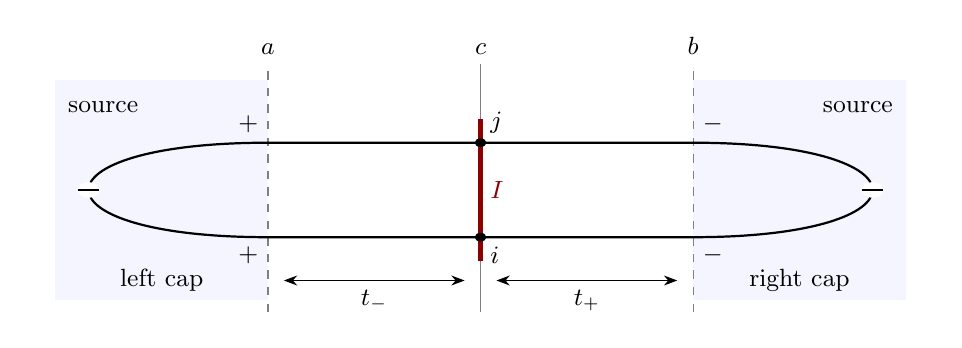
\begin{tikzpicture}[x=1.35cm,y=1cm,>=Stealth,
    every node/.style={font=\small}]
  \fill[blue!4] (-4,-1.4) rectangle (-2,1.4);
  \fill[blue!4] (2,-1.4) rectangle (4,1.4);
  \draw[dashed,gray] (-2,-1.55)--(-2,1.6);
  \draw[dashed,gray] (2,-1.55)--(2,1.6);
  \draw[gray] (0,-1.55)--(0,1.6);
  \draw[line width=2pt,red!55!black] (0,-.9)--(0,.9);
  \draw[thick] (-2,.6)--(2,.6)
    .. controls (4.25,.6) and (4.25,-.6) .. (2,-.6)
    --(-2,-.6)
    .. controls (-4.25,-.6) and (-4.25,.6) .. (-2,.6);
  \fill[white] (-3.6875,0) circle (.10);
  \draw[thick] (-3.7875,0)--(-3.5875,0);
  \fill[white] (3.6875,0) circle (.10);
  \draw[thick] (3.5875,0)--(3.7875,0);
  \fill (0,.6) circle (.055);
  \fill (0,-.6) circle (.055);
  \node[above left] at (-2,.6) {$+$};
  \node[below left] at (-2,-.6) {$+$};
  \node[above right] at (2,.6) {$-$};
  \node[below right] at (2,-.6) {$-$};
  \node[above right] at (0,.6) {$j$};
  \node[below right] at (0,-.6) {$i$};
  \node[right,red!55!black] at (0,0) {$I$};
  \node at (-3,-1.15) {left cap};
  \node at (3,-1.15) {right cap};
  \node[above] at (-2,1.6) {$a$};
  \node[above] at (0,1.6) {$c$};
  \node[above] at (2,1.6) {$b$};
  \node[above] at (-3.55,.86) {source};
  \node[above] at (3.55,.86) {source};
  \draw[<->] (-1.85,-1.15)--(-.15,-1.15);
  \draw[<->] (.15,-1.15)--(1.85,-1.15);
  \node[below] at (-1,-1.15) {$t_-$};
  \node[below] at (1,-1.15) {$t_+$};
\end{tikzpicture}
\caption{A same-loop contribution to the insertion. The selected cap arches
carry two sources: the endpoint signs are \(++\) at the left seam and
\(--\) at the right seam. The two sinks \(i,j\) lie in the middle
interval \(I\). The insertion changes the permitted color assignments
while preserving the uncolored loop. The positive propagation widths
\(t_-\) and \(t_+\) control the sum over mode states.}
\label{fig:two-particle-insertion}
\end{figure}


\begin{lemma}[Sandwiched insertion]
\label{lem:sandwiched-insertion}
Let $\mathcal T_-$ and $\mathcal T_+$ be the two-replica transfers from
$a$ to $c$ and from $c$ to $b$, with column lengths $t_-$ and $t_+$.
For the fixed positive widths above, so that $t_\pm\ge\eta n$ for some
$\eta>0$ and all sufficiently small meshes,
\begin{equation}
 \bigl\|s^{-2(t_-+t_+)}
       \mathcal T_+\mathcal O_I\mathcal T_-\bigr\|
       \le C\left(\frac{|S(I)|}{n}\right)^2.
 \label{eq:sandwiched-insertion}
\end{equation}
Consequently, uniformly over the cap-local weights $\lambda(A)\in[0,1]$,
\begin{equation}
 \frac{\bigl|\langle V_R,
       \mathcal T_+\mathcal O_I\mathcal T_-V_L\rangle\bigr|}
      {Z_{\rm dd}}
 \le C_M\left(\frac{|S(I)|}{n}\right)^2.
 \label{eq:marked-contraction-bound}
\end{equation}
\end{lemma}

\begin{proof}
Use the real orthogonal singular-mode basis at the middle seam supplied
by Lemma~\ref{lem:spectrum}; it is the same for both replicas.  Write
its change-of-basis matrix as $Q$, and put
\[
 P_I=Q^T\1_{S(I)}Q.
\]
Here $\1_{S(I)}$ is the diagonal orthogonal projection onto the indicated
site coordinates.
For a removed mode pair $R=\{r,s\}$, $r<s$, and an added mode pair
$T=\{u,v\}$, $u<v$, the coefficient of pair deletion in the first factor
and pair creation in the second is
\begin{equation}\label{eq:insertion-minor}
 \sum_{\substack{i<j\\i,j\in S(I)}}
       \det Q_{\{i,j\},R}\,\det Q_{\{i,j\},T}
 =\det (P_I)_{R,T}.
\end{equation}
All pairs use increasing order; the equality is the two-by-two
Cauchy--Binet identity.  For fixed input and output occupation states,
the removed pair is their set difference in the first factor and the
added pair is their set difference in the second.  Thus a nonzero
matrix entry uses exactly one coefficient in
\eqref{eq:insertion-minor}, multiplied by the occupation-state sign.
The delocalization bound $|Q_{ir}|\le C/\sqrt n$ gives
\[
 |(P_I)_{rs}|\le C^2\frac{|S(I)|}{n},
 \qquad
 |(\mathcal O_I)_{\alpha\beta}|
       \le 2C^4\left(\frac{|S(I)|}{n}\right)^2.
\]

We must also control the sum over mode states.  For a two-replica mode
state $\mu=(J,K)$, set
\[
 d_\pm(\mu)=w_{t_\pm}(J)w_{t_\pm}(K),
\]
using the normalized single-replica weights of Lemma~\ref{lem:spectrum}.
Equation~\eqref{eq:all-state-sum}, which includes the zero mode, gives
$\sum_\mu d_\pm(\mu)\le C_\eta^2$, even when the sums run over all
particle sectors.  In the compatible singular bases the normalized
transfers are diagonal, so the sandwiched matrix has entries
$d_+(\nu)(\mathcal O_I)_{\nu\mu}d_-(\mu)$.  Consequently
\[
 \begin{split}
 \bigl\|s^{-2(t_-+t_+)}\mathcal T_+\mathcal O_I\mathcal T_-\bigr\|
 &\le\sum_{\nu,\mu}d_+(\nu)
             |(\mathcal O_I)_{\nu\mu}|d_-(\mu)\\
 &\le 2C^4\left(\frac{|S(I)|}{n}\right)^2
       \left(\sum_\nu d_+(\nu)\right)
       \left(\sum_\mu d_-(\mu)\right).
 \end{split}
\]
The operator norm is bounded by the entrywise absolute sum, and the
bounded state sums prove~\eqref{eq:sandwiched-insertion}.
The displayed bounds on $\|V_L\|,\|V_R\|$ and the partition comparison in
Lemma~\ref{lem:cap-comparison} now prove
\eqref{eq:marked-contraction-bound}.
\end{proof}

The analytic estimate supplies a factor $|S(I)|^2$ for every permitted
choice of weights.  To use it for a probability, we must choose the
weights so that the full signed contraction is nonnegative and detects
the event we want to exclude.  We now compute its contributions before
making that choice.

\subsection{The pointwise color calculation}

Fix an ordinary uncolored double-dimer configuration $\omega$.  Each
nondoubled loop has two assignments of its alternating edges to the
two matchings; doubled edges have only one.  For each selected pair of
cap arches and each sink pair $i<j$ in $S(I)$, count the modified color assignments
satisfying the two source rules and the two insertion rules.  Multiply
by~\eqref{eq:insertion-parity}, divide by the ordinary number of
assignments, and multiply by the two cap weights $\lambda$.  Sum over
the choices, and define the result to be $X^\lambda_{M,I}(\omega)$;
set it to zero on $E_M^c$.  Lemma~\ref{lem:marked-cap} gives the exact
identity
\begin{equation}\label{eq:observable-contraction}
 \EE X^\lambda_{M,I}
 =\frac{\langle V_R,\mathcal T_+\mathcal O_I\mathcal T_-V_L\rangle}
        {Z_{\rm dd}}.
\end{equation}

To compute this color ratio, cut the uncolored configuration at the
middle seam $x=c$.  A marked loop not reaching that seam has no possible
sink and contributes zero.  Otherwise the selected left cap arch lies
in a unique arch of the same loop in $\{x<c\}$.  Direct its two branches
away from the source.  Ordinary strands propagate these directions to
the middle seam, where both branches leave the left half-plane.
The induced endpoint signs are therefore $++$.  On the right the same
argument gives $--$, because both branches leave $\{x>c\}$.
An unmarked middle-seam arch has one entrance and one exit, hence
opposite endpoint signs.

Several choices of a remote eligible arch can lie on the same
middle-seam arch.  We keep them as separate marked choices, each with
its own weight.  Moving a source along that arch changes no
intersection with $I$.  Thus the color calculation below applies to
each remote choice and preserves its multiplicity when we sum.

Rank the singly occupied edges along the whole middle seam, and give
rank $r$ the alternating sign $\sigma_r=(-1)^r$.  Formula
\eqref{eq:insertion-parity} becomes
\begin{equation}
 -\sigma_i\sigma_j
 \label{eq:rank-insertion-sign}
\end{equation}
when $i,j$ now denote the two ranks.  On any one simple loop these rank
signs agree with oriented intersection signs up to a common sign.
To see why other loops do not affect this assertion, take two seam
hits of the chosen loop.  They have the same inside/outside relation
to every other disjoint loop.  Each such loop therefore contributes an
even number of hits between them.  After these even contributions are
removed, the assertion is the usual alternation of entering and
leaving a Jordan domain along a line.

\begin{lemma}[One or two marked loops]
\label{lem:color-contractions}
Fix one eligible mark in each cap, before multiplying their weights.
\begin{enumerate}[label=\textnormal{(\roman*)}]
 \item If both marks lie on one loop, let $u,v$ be the intersection
 numbers with $I$ of its two mark-to-mark arcs, both oriented from the
 left mark to the right mark.  Its summed signed color ratio is
 $uv/2$.  This is nonnegative, and is at least $1/2$ when $u,v\ne0$.
 \item If the marks lie on distinct loops $g,g'$, put
 \[
 t_g=\sum_{\text{hits of }g\text{ in }I}\sigma_r.
 \]
 Their summed signed color ratio is $-t_gt_{g'}/4$.  The number $t_g$
 is zero unless $g$ separates the endpoints of $I$, in which case it
 is $1$ or $-1$.
\end{enumerate}
\end{lemma}

\begin{proof}
One can express the color rules using signs $x_r^L,x_r^R\in\{-1,1\}$
on the two sides of each single middle-seam hit.  An unmarked arch
requires opposite signs at its ends.  A marked left arch fixes both
signs to $+1$, and a marked right arch fixes both to $-1$.  Ordinary
seam gluing requires $x_r^L=x_r^R$, whereas a selected sink fixes
$(x_r^L,x_r^R)=(+1,-1)$.  On an ordinary loop these constraints leave
one free binary choice; once a source is prescribed, propagation fixes
every remaining sign whenever the constraints are compatible.

At a source the two oriented strands point away from the mark;
at a sink they point toward it.  Continuing the assignments around a
loop shows that sources and sinks must alternate.  On a loop with two
sources, the sink pair is therefore admissible precisely when it puts
one sink on each of the two mark-to-mark arcs.  It then prescribes one
assignment instead of the two ordinary choices.  The two arcs have
opposite directions relative to any coherent orientation of the
whole loop, canceling the minus sign in
\eqref{eq:rank-insertion-sign}.  Summing the remaining products of
crossing signs yields $uv/2$.

The whole-loop intersection number, in the orientation of the first
arc, is $u-v$, so~\eqref{eq:whole-loop-index} implies $|u-v|\le1$.
Because $u,v$ are integers, their product is nonnegative, and is at
least one if neither vanishes.

For two distinct marked loops there must be one sink on each.  The
colors of each marked loop are then fixed, replacing four ordinary
choices by one.  Summing~\eqref{eq:rank-insertion-sign} gives
$-t_gt_{g'}/4$.  The rank-sign observation before the lemma identifies
$t_g$, up to a sign, with the whole-loop intersection number.  This
number vanishes exactly when the endpoints of $I$ have the same
inside/outside status with respect to $g$.
\end{proof}

For a precise parity identity, order the endpoints $A,B$ of $I$ in the
increasing seam direction, and let $d(g)$ be the number of loops strictly
enclosing $g$.  Start rank numbering at the first hit of the whole seam,
so that the region before all hits is exterior to every loop.  Then
\begin{equation}
 t_g=-(-1)^{d(g)}
 \bigl(\1_{\{B\in\operatorname{Int}(g)\}}
       -\1_{\{A\in\operatorname{Int}(g)\}}\bigr).
 \label{eq:rank-nesting-depth}
\end{equation}
Indeed at a hit entering $g$, the nesting parity just before the hit is
$d(g)$, and at a hit leaving $g$ it is $d(g)+1$.  Since
$\sigma_r=(-1)^r$, summing these signed changes telescopes to
\eqref{eq:rank-nesting-depth}, regardless of how often $g$ hits the seam.

The loops separating the endpoints of $I$ form at most two nested
chains, one around either endpoint, with their common ancestors
omitted.  Order each chain from its outermost loop inward.  The signs
$t_g$ alternate along each chain.  If both chains are nonempty, the
two outermost signs are opposite.  Successive members of either chain
have ancestor depths differing by one.  The two outermost members, when
both exist, border the same common-ancestor region and have equal
depths, but the endpoint differences in
\eqref{eq:rank-nesting-depth} have opposite signs.  Common ancestors
change both depth parities equally; other nonseparating loops do not
affect the identity.  Endpoints outside the rectangle are permitted in
this description.

\subsection{Nested arches and positivity}

Only loops separating the endpoints of $I$ contribute to the
different-loop sum, since the other loops have $t_g=0$.  For such a
loop $g$, let
\[
 U_g=\sum_{\substack{A\text{ eligible left arch}\\A\subset g}}\lambda(A),
 \qquad
 V_g=\sum_{\substack{A\text{ eligible right arch}\\A\subset g}}\lambda(A).
\]
These totals still depend on the weights to be chosen; empty sums are
zero.  The total contribution from marks on distinct
loops is, by Lemma~\ref{lem:color-contractions},
\begin{equation}
 -\frac14\sum_{g\ne g'}U_gV_{g'}t_gt_{g'}.
 \label{eq:different-loop-sum}
\end{equation}
Individual summands can be negative: two loops whose positions in a
chain differ by two have the same sign $t_g$.  We choose the weights
so that the total mark weights decrease by a factor of at least two
along either nesting chain.  The resulting alternating sums will
control the complete expression~\eqref{eq:different-loop-sum}.

The weights must still be determined within each cap.  For an eligible
arch $A$, let $b(A)$ count the eligible arches in that cap whose
endpoints strictly span those of $A$ along its seam.  Choose
\begin{equation}
 \lambda(A)=w(A):=(2M)^{-b(A)}.
 \label{eq:arch-weight}
\end{equation}
On $E_M$ every such weight belongs to $[q_M,1]$, where
\begin{equation}
 q_M=(2M)^{-(M-1)}.
 \label{eq:minimum-arch-weight}
\end{equation}
From now on $U_g,V_g$ use this choice, and write
$X_{M,I}=X^w_{M,I}$.  Every nonzero $U_g$ or $V_g$ is at least $q_M$,
because it contains at least one eligible-arch weight.
To connect the endpoint nesting chains to these
cap weights, we show that every eligible arch of an inner separating
loop is spanned by an eligible arch of the outer loop.  That additional
spanning arch supplies a factor $1/(2M)$; the cutoff of $M$ arches will
then give the required factor $1/2$ for the total weights.

\begin{lemma}[Decrease of the cap weights]
\label{lem:cap-weight-decrease}
On $E_M$, if a separating loop $g'$ lies inside another separating
loop $g$, then
\[
 U_{g'}\le\tfrac12 U_g,
 \qquad V_{g'}\le\tfrac12 V_g.
\]
In particular a zero outer weight forces all deeper weights in that
cap to be zero.
\end{lemma}

\begin{proof}
Consider an eligible arch $A'$ of $g'$ in one cap.  Since $g$ separates
the endpoints of the middle interval, it reaches the middle seam and
is not contained in the cap half-plane.  Its portions in that
half-plane are disjoint arches.  Each such arch $A$, closed by the
interval between its seam endpoints, bounds a Jordan disk $D_A$.
Inside the open cap half-plane, the indicator of the interior of $g$
is the parity sum of the indicators of these disks: the two sides
have the same boundary there and both vanish sufficiently far away.
An interior point of $A'$ therefore belongs to at least one $D_A$.
The whole interior of $A'$ stays in that disk, since it cannot cross
$A$ or the cap seam.  Thus the endpoints of $A$ strictly span those of
$A'$.

The disk $D_A$ reaches no deeper into the cap than its boundary arch.
Since $A'$ reaches the prescribed deep region, $A$ also reaches it and
is eligible.  Every eligible arch spanning $A$ also spans $A'$, and
$A$ itself supplies one additional spanning arch.  Consequently
\[
 b(A')\ge b(A)+1,
 \qquad w(A')\le\frac{w(A)}{2M}.
\]
There are at most $M$ eligible inner choices.  Bounding each containing
outer weight by the largest outer weight gives
\[
 \sum_{A'\subset g'}w(A')
 \le\tfrac12\max_{A\subset g}w(A)
 \le\tfrac12\sum_{A\subset g}w(A).
\]
This proves the assertion independently in the two caps.
\end{proof}

\begin{lemma}[Two alternating chains]
\label{lem:two-chain-positivity}
Suppose a finite family consists of at most two chains, each ordered
from outside inward.  Give its members signs $t_g\in\{-1,1\}$ which
alternate in either chain and have opposite outermost signs when
both chains are present.  Let $U_g,V_g\ge0$ decrease by a factor of at
least two at each step inward.  Then the expression
\eqref{eq:different-loop-sum} is nonnegative.  If every positive $U_g$
or $V_g$ is at least $q>0$ and there are distinct $g,g'$ with $U_gV_{g'}>0$, the
expression is at least $q^2/16$.
\end{lemma}

\begin{proof}
Within one chain write its indices as $1,\ldots,k$.  Group the terms
by their outer member to obtain
\[
 \frac14\sum_{i=1}^{k-1}
 \left[
 U_i\sum_{j>i}(-1)^{j-i+1}V_j+
 V_i\sum_{j>i}(-1)^{j-i+1}U_j
 \right].
\]
Each inner alternating sum is nonnegative and is at least half its
first term, since successive magnitudes decrease by a factor of at
least two.  If a particular product $U_iV_j$ or $V_iU_j$ with $i<j$ is
positive, the appropriate first term at $i+1$ is positive as well.
That group then contributes at least $q^2/8$.

Between the two chains the sum is
\[
 -\frac14\left[
 \left(\sum_{g\in C_1}U_gt_g\right)
 \left(\sum_{g\in C_2}V_gt_g\right)
 +
 \left(\sum_{g\in C_2}U_gt_g\right)
 \left(\sum_{g\in C_1}V_gt_g\right)
 \right].
\]
Each weighted alternating sum is zero or has its chain's outermost sign, and has
absolute value at least half its outermost weight.  The signs of the
two chains are opposite, so both displayed products give nonnegative
contributions after the leading minus sign.  A positive product
between distinct chains forces the relevant outermost weights to be
at least $q$, giving a contribution of at least $q^2/16$.
\end{proof}

We can now finish the detection argument.  Lemma~\ref{lem:color-contractions}
makes every same-loop term of $X_{M,I}$ nonnegative.
Lemmas~\ref{lem:cap-weight-decrease} and~\ref{lem:two-chain-positivity}
make its complete different-loop term nonnegative.  Thus
\begin{equation}
 X_{M,I}\ge0.
 \label{eq:positive-observable}
\end{equation}

If condition (i) of Proposition~\ref{prop:rectangle-short} occurs, each
deep endpoint of the tested arc lies in an eligible arch of its cap.
Select those two arches.  Moving the endpoints to the marks inside
these arches changes no intersection with $I$, since the arches stay
strictly on their respective sides of the middle seam.  If the tested
arc has intersection number $a$ and the whole loop has number $e$,
the two mark-to-mark sums have product $a(a-e)$.  Here $a\ne0,e$ and
$e\in\{-1,0,1\}$, so this product is a positive integer.  The weighted
same-loop term is at least $q_M^2/2$.

Suppose instead that condition (ii) occurs and no tested arc gives
condition (i).  Each of its two nonzero arc sums must then equal the
corresponding whole-loop sum.  The two loops separate the endpoints
of $I$ and each has an eligible arch in each cap.  In particular there
is a distinct pair with $U_gV_{g'}>0$.  Their full different-loop sum
is at least $q_M^2/16$.  We have proved the pointwise bound
\begin{equation}
 X_{M,I}\ge\frac{q_M^2}{16}\,
 \1_{E_M\cap\{\textnormal{condition (i) or (ii) holds on }I\}}.
 \label{eq:pointwise-detection}
\end{equation}

\subsection{Summing the short intervals}

\begin{proof}[Proof of Proposition~\ref{prop:rectangle-short}]
For a partition interval $I$, combine
\eqref{eq:marked-contraction-bound},
\eqref{eq:observable-contraction}, and
\eqref{eq:pointwise-detection} to obtain
\[
 \PP\bigl(E_M\cap\{\text{a violation on }I\}\bigr)
 \le C_M\left(\frac{|S(I)|}{n}\right)^2.
\]
The transverse size of the limiting rectangle is positive and fixed,
so an interval of length at most $h$ contains at most $C(h/\delta+1)$
sites and $n\ge c/\delta$.  Consequently
\[
 \frac{|S(I)|}{n}\le C(h+\delta).
\]
There are at most $C_J/h$ intervals.  The union bound therefore yields
\begin{equation}
 \PP(B_{\delta,h})
 \le\PP(E_M^c)+C_M\frac{(h+\delta)^2}{h}.
 \label{eq:short-union-bound}
\end{equation}
For each fixed $M$, first take the upper limit as $\delta\downarrow0$
and then let $h\downarrow0$.  The remaining bound is
$\limsup_{\delta\downarrow0}\PP(E_M^c)$, which tends to zero as
$M\to\infty$ by~\eqref{eq:cap-cutoff-tight}.  This proves the stated
order of limits.  The argument used only the sites actually contained
in an interval; endpoints outside the rectangle and intervals
truncated by a transverse side cause no change.
\end{proof}

\section{Localization and compactness of the curves}
\label{sec:localization}

The rectangle estimates must be transferred to the specified half-plane
measure before they can control its loops.  We first couple matching
states in a bounded window, uniformly in the lattice mesh.  This coupling
does not determine connections outside the window.  Nevertheless, it
preserves the local directed paths needed for both estimates.  We then
use the traversal bound to obtain compactness in the fixed disk
coordinates, retaining every nonconstant limiting loop.

\subsection{A uniform comparison with finite rectangles}

Write $\mathcal R_{\delta,R}$ for a Temperleyan rectangle whose coarse
bottom side is at height $\delta$, whose other sides are within $O(\delta)$
of $x=-R$, $x=R$, and $y=R$, and whose lower left coarse corner is deleted.
Rounding the sides to the coarse grid gives odd numbers of fine-grid
vertices in both directions.  The precise rounding will be immaterial.
Agreement of matching states on a set means agreement on every edge
having at least one endpoint in that set.

\begin{proposition}[Uniform localization]
\label{prop:localization}
Let $K$ be a bounded closed subset of $\overline{\HH}$ and let $\eps>0$.
There is an $R<\infty$ such that, for every sufficiently small $\delta$,
the two independent half-plane matchings can be coupled with two
independent uniform matchings of $\mathcal R_{\delta,R}$ so that both
matching states agree on $K$ with probability at least $1-\eps$.
\end{proposition}

Here is the finite graph to which we apply the Temperley
correspondence~\cite[Theorem~1]{KPW}. Let $G$ be the coarse rectangular
grid of mesh $2\delta$, including its lower left corner $r$, and let
$G^*$ be its plane dual, with exterior vertex $f_\infty$. The fine-grid
vertices are the vertices of $G$, its edge midpoints, and its bounded
face centers. A midpoint is joined to the endpoints of its coarse edge
and to its incident bounded face centers. Deleting $r$ gives exactly
$\mathcal R_{\delta,R}$; the exterior face-node is omitted from this
matching graph.

A spanning tree $T$ of $G$ is directed toward $r$. Its complementary
dual tree $T^*$ is directed toward $f_\infty$. Each remaining primal
vertex is matched to the midpoint of its outgoing edge in $T$.
Each bounded face center is matched to the midpoint of the primal
edge crossed by its outgoing edge in $T^*$. The corner $r$ is incident
with the exterior face, so the
correspondence is a bijection. All edge weights are one: uniform
matchings correspond to uniform primal trees and, by complementation,
to uniform dual trees. In $G^*$ we retain a separate edge to
$f_\infty$ for every primal boundary edge, including parallel edges.

Wilson's algorithm~\cite{Wilson,PW} samples this finite dual tree by
loop-erasing walks stopped on the tree already drawn, starting with
$f_\infty$. Each walk chooses uniformly among the four edge options at
a bounded face. A proposed step crossing a primal boundary edge is
absorbed at $f_\infty$, and we retain that boundary edge as its physical
contact. Theorems~13 and~16 of~\cite{PW} permit any fixed order of
starting sites. We will confine the dual paths needed near $K$ and
then recover the primal directions from the cycles they determine.
The following walk estimate supplies the uniform attachment
probability used in that confinement.

\begin{lemma}[Attachment near an explored branch]
\label{lem:walk-attachment}
Fix $1\le C_0<\infty$.  There are constants $C_1>C_0$ and $p>0$ with the
following property.  Let a square-lattice walk have mesh $a_0$, start at
$x$ above a horizontal killing boundary, and let $a\ge a_0$.
Suppose an already explored nearest-neighbor path starts within distance
$C_0a$ of $x$ and runs to that boundary.  The probability that the walk
hits the path or the killing boundary before leaving $B(x,C_1a)$ is at
least $p$.  The constants are independent of the path, the mesh, and
the distance of $x$ from the boundary.
\end{lemma}

\begin{proof}
Adjoin the closed lower half-plane to the explored path.  The resulting
connected set meets $B(x,C_0a)$ and extends outside every larger ball.
It is therefore enough to give the unrestricted walk a fixed positive
probability of tracing a closed circuit surrounding $B(x,C_0a)$ before
leaving $B(x,C_1a)$.  If such a circuit crosses the killing boundary,
the killed walk has already stopped, which is also a success.

Here is a concrete way to force an actual circuit, rather than just a
near-return.  At unit scale, first cross a small rectangle to the right
of the inner ball horizontally.  Follow a thin polygonal corridor once
around the inner ball and return to cross that same rectangle vertically.
The two crossings meet by planarity; the intervening part of the trace
contains a closed curve of nonzero winding around the inner ball.  All
corridors lie in a fixed larger ball.  The event can be specified by
finitely many crossings with fixed positive margins.  Brownian motion
has positive probability of following these corridors, and the
invariance principle gives a uniform lower bound when $a/a_0$ is large.
Here the polygonal square walk has mean-zero increments with covariance
$\tfrac12 I$. Scalar Donsker convergence
\cite[Theorems~8.1.4 and~8.1.11]{Durrett} gives tightness of its two
coordinate processes; the vector central limit theorem for disjoint
increment blocks identifies their joint limit as planar Brownian
motion with covariance $\tfrac12 tI$. The prescribed corridor event
contains a uniform open neighborhood of a continuous polygonal route
with these crossings and positive margins. Its Brownian probability is
positive, so the open-set Portmanteau bound yields the claimed lower
bound. This comparison does not depend on the absorbing path.
For bounded $a/a_0$, force an appropriate finite square-lattice circuit;
after enlarging $C_1$, only boundedly many steps and finitely many local
lattice configurations are involved.  Decreasing the lower bound to
cover these cases gives $p>0$ for all scales.  A separating circuit must
meet the connected absorbing set, proving the assertion.
\end{proof}

\begin{proof}[Proof of Proposition~\ref{prop:localization}]
We first compare one matching in $\mathcal R_{\delta,R}$ with one in a
larger rectangle.  Choose a fixed rectangular window $W_\infty$ containing
$K$ and a neighborhood of it. For every coarse edge whose midpoint is
incident to a fine-grid edge having an endpoint in $K$, explore the
dual paths from all bounded faces incident with that coarse edge.
These are the finite endpoints of its dual edge; they lie within
$O(\delta)$ of $K$ and hence in $W_\infty$ for small $\delta$.
The explored paths determine the relevant dual edges and, through the
fundamental cycles used below, the relevant primal directions.
The walk has mesh $2\delta$ until it is absorbed. At the bottom we
record the crossed primal edge, using the boundary-contact convention
above.

\paragraph{Nets and shrinking windows.}
We explore coarse nets before finer ones. Each finer starting site
will then be close to a previously drawn path to the bottom. If the
net spacing is $a_j$ and the allowed excursion is $b_j$, a walk must
miss order $b_j/a_j$ opportunities to attach before making such an
excursion. We choose these scales so that the failure probabilities
remain summable after counting all net sites.
Put $a_j=2^{-j}$ and $b_j=B2^{-j/2}$, where $B>0$ is fixed.  Enlarge
$W_\infty$ horizontally and upward by $\sum_{\ell>j}b_\ell$ to obtain
$W_j$.  Thus $W_{j-1}$ has a margin $b_j$ around $W_j$, apart from the
common bottom boundary.  In $W_j$ choose a dual-lattice net $N_j$ of
spacing comparable to $a_j$, including sites next to the bottom.  It
has at most $Ca_j^{-2}$ sites and covers $W_j$ within distance $Ca_j$.
Run Wilson's algorithm from these nets in increasing order, starting
with $j=0$ and skipping sites already in the tree.  Stop at the unique
level $J=J(\delta)$ for which $2\delta\le a_J<4\delta$, and take every
dual site in $W_J$.  Its cardinality is still $O(4^J)$.  Thus every
required site has been explored.

Suppose all branches already drawn end on the bottom.  At a late level
$j$, declare an error if a new walk travels distance $b_j/3$ from its
start before attaching.  Before this happens, the walk stays inside
$W_{j-1}$.  At any intermediate location there is a site of $N_{j-1}$
within $Ca_{j-1}=O(a_j)$, together with its previously drawn path to the
bottom.  Lemma~\ref{lem:walk-attachment} gives a uniformly positive
chance of attachment before the walk leaves a ball of radius $Da_j$.
Before the declared error, the walk is at least $2b_j/3$ from the
other three sides of $W_{j-1}$. Since $Da_j/b_j\to0$, these test balls
stay within those sides for all sufficiently large $j$; they may
cross the killing boundary.
By the strong Markov property at successive ball exits,
traveling distance $b_j/3$ without attachment requires at least
$cb_j/a_j$ failed trials.  Consequently its conditional probability is
at most
\begin{equation}
 C\exp(-c b_j/a_j)\le C\exp(-c2^{j/2}).
 \label{eq:wilson-net-tail}
\end{equation}
Independence between these trials or between different walks is not
needed.  The conditional lower bound on attachment suffices.

Summing over all starts at levels above $j_0$ bounds the late-level
error by
\begin{equation}
 C\sum_{j>j_0}4^j\exp(-c2^{j/2}),
 \label{eq:wilson-net-sum}
\end{equation}
uniformly in $\delta$.  This tends to zero as $j_0\to\infty$.
The final all-sites level obeys the same estimate.

\paragraph{The finitely many early walks.}
Fix $j_0$ so that \eqref{eq:wilson-net-sum} is small.  There are boundedly
many starts up to that level, all in a fixed bounded window.  An
unrestricted square-lattice walk started at height at most $H$ obeys,
in diffusive time units,
\[
 \PP(\tau_{\mathrm{bottom}}>T)
 \le \frac{C(H+\delta)}{\sqrt T},
 \qquad
 \PP\left(\max_{s\le T}|X_s-X_0|>A\right)
 \le \frac{CT}{A^2}.
\]
The first inequality is the one-dimensional hitting estimate for the
lazy vertical coordinate; the second is the martingale maximal
inequality.  Choosing first $T$ and then $A$ makes the probability of
leaving a large window before hitting the bottom arbitrarily small,
uniformly for fine meshes.  A Wilson walk stops no later if it first
hits an earlier branch.  A union bound therefore confines all early
walks with arbitrarily high probability.

Choose $R$ to contain this large window and the net windows with their
allowed excursions.  On the event of no early or late error, every
required dual branch lies in $\mathcal R_{\delta,R}$ and reaches the
wired exterior through its bottom side.  Use the same walk increments
in $\mathcal R_{\delta,R}$ and any larger exhausting rectangle.
Their explorations agree exactly on this event.  Adding the remaining
Wilson branches does not alter paths already drawn.

\paragraph{Primal directions.}
It remains to recover more than dual edge membership.  The matching
also uses the directions of primal tree edges toward the deleted
corner.  Let $e$ be a primal tree edge relevant to $K$.  Its crossing
dual edge $e^*$ is absent from the dual tree.  Adding $e^*$ creates a
dual fundamental cycle, which separates the two components of the
primal tree with $e$ removed.  The direction of $e$ is from the
component not containing the root to the component containing it.
The dual branches from the endpoints of $e^*$ determine this cycle;
these were among the required explored branches.

If the cycle avoids the wired exterior, it is contained in the bounded
exploration window, and the remote corner root lies outside it.  If it
uses the wired exterior, all its exterior contacts are on the bottom
within that same bounded window.  Represent the exterior part just
below the bottom, between the two contacts.  The cycle cuts off a
bounded pocket along that bottom interval; the remote corner root is
outside the pocket.  A bottom primal edge is treated identically, with
one contact supplied by $e^*$ itself.  No contact on a remote side or
top can occur on the confinement event.  Thus the component containing
the root, and hence every required primal direction, is the same in
the two rectangles.  Planar duality and the Temperley correspondence
now give identical matching states on $K$.

For each fixed mesh the number of matching states on $K$ is finite.
Let the comparison rectangle exhaust $\HH$ and take a subsequential
limit of the coupled window laws.  Its second marginal is the specified
half-plane local limit, and the agreement bound persists.  Extending
this window coupling by the respective conditional laws gives the
coupling of full matchings.  Finally use two independent copies of the
construction, with half the allotted error for each copy.  This
preserves independence within each pair and proves the proposition.
\end{proof}

\subsection{The two geometric consequences in the half-plane}

We next state exactly what is preserved when the connections outside a
window change.  A directed loop always has the orientation fixed by the
matching labels: first-matching edges go from black to white and
second-matching edges from white to black.  For a directed path portion
$\alpha$ and a transverse segment $I$, retain the notation $\iota_I(\alpha)$ for its
signed intersection sum.  The path endpoints are kept off the test
line, and the segment endpoints off the lattice graph.  A fixed line
between lattice columns or rows may be used as a seam; it need not
bisect the crossed edges.

\begin{corollary}[Local traversal counts]
\label{cor:local-crossings}
Fix a bounded window $K\subset\overline{\HH}$ and two distinct parallel
coordinate lines.  For horizontal lines assume both have positive
height.  The maximum total number of parameter-disjoint portions of
half-plane double-dimer cycles that lie in $K$ and traverse from one
line to the other, in either direction, is tight as $\delta\downarrow0$.
\end{corollary}

\begin{proof}
Apply Proposition~\ref{prop:localization} to a fixed neighborhood of
$K$.  On its agreement event, all such portions are also portions of
rectangle cycles.  Their connections
outside $K$ may differ, but their crossing paths and their
parameter-disjointness do not.  Their number is therefore bounded by
the rectangle traversal count of
Proposition~\ref{prop:rectangle-crossings}.  Take $R$ large enough that
both cuts have positive longitudinal room to the rectangle ends.
For horizontal cuts this uses their positive heights; for vertical
cuts it follows by increasing $R$.  The coupling error is arbitrary,
so the rectangle tightness gives the assertion.  If an original cut
contains lattice vertices, use two slightly inward seams instead:
every traversal of the original slab crosses the inward seams, whose
limiting separation is unchanged.
\end{proof}

\begin{proposition}[Local exclusion of opposite intersection signs]
\label{prop:local-opposite}
Let $u$ be either the horizontal or vertical coordinate, let
$L=\{u=c\}$ be a test line, and let $J\subset L$ be a bounded segment.
If $u$ is the vertical coordinate, assume $c>0$.  Fix a bounded window
$K\subset\overline{\HH}$ and buffers $\rho_-,\rho_+>0$.  Deterministically partition $J$
into $O(h^{-1})$ intervals of length at most $h$, with endpoints off the
graph.  Let $E_{\delta,h}$ be the event that, for one of these intervals
$I$, one directed half-plane cycle has two portions $\alpha,\beta$
contained in $K$ such that each portion has one endpoint in
$\{u\le c-\rho_-\}$ and the other in $\{u\ge c+\rho_+\}$, and
\[
 \iota_I(\alpha)\iota_I(\beta)<0.
\]
Then
\begin{equation}
 \lim_{h\downarrow0}\limsup_{\delta\downarrow0}
 \PP(E_{\delta,h})=0.
 \label{eq:local-opposite-limit}
\end{equation}
For a vertical line $L$, the segment may reach or extend below the
bottom boundary.  Test lines are chosen off lattice vertices; the
same estimate holds for seam perturbations of order $\delta$.
\end{proposition}

\begin{proof}
Fix a coupling error $\eps>0$ and apply
Proposition~\ref{prop:localization} to a neighborhood of $K$.
On its agreement event, both directed portions remain rectangle
paths with exactly the same signs, because the two matching labels
are preserved.  There are two possibilities for their new connections.
If the portions belong to distinct rectangle cycles, their two nonzero
indices give the second forbidden event in
Proposition~\ref{prop:rectangle-short}.  If they belong to the same
rectangle cycle $g$, its whole-cycle index satisfies
$\iota_I(g)\in\{-1,0,1\}$ by the Jordan curve theorem.  Two opposite nonzero
integers cannot both equal $\iota_I(g)$; at least one portion therefore
gives the first forbidden event of that proposition.

The rectangle can be chosen with all required cuts longitudinally
interior.  For a horizontal middle line, a nonempty event already
requires endpoints below it; take its lower cap between those
endpoints and the middle line, at positive height.  For a vertical
middle line there is no corresponding restriction at the bottom:
the test interval is transverse, and
Proposition~\ref{prop:rectangle-short} permits its truncation at a
transverse end.  Rotation and reflection give the same argument in
both coordinate directions and for either direction of each portion.
Consequently
\[
 \lim_{h\downarrow0}\limsup_{\delta\downarrow0}
 \PP(E_{\delta,h})\le\eps.
\]
Let $\eps\downarrow0$.  Rounding a cut by $O(\delta)$ leaves fixed
positive buffers and longitudinal room, and the rectangle bounds are
uniform under this rounding.  Alternatively, along any prescribed
mesh sequence one may choose fixed test lines and endpoints avoiding
all its lattice sites, as we shall do in Section~\ref{sec:identification}.
\end{proof}

\subsection{From local traversals to compactness in the disk}

We now use Corollary~\ref{cor:local-crossings} to control parametrizations,
not merely the number of loops. The use of crossing control and
multiscale time changes to obtain compactness follows the strategy of
Aizenman--Burchard~\cite[Lemma~2.4 and Section~4]{AB}. We use the direct
partition construction below, which requires only our fixed-scale
traversal tightness. For a collection of parametrized loops
in $\overline{\DD}$, let $N_\eta$ be the largest total number of
parameter-disjoint portions whose two endpoints have Euclidean
distance greater than $\eta$.  Parameter interiors are disjoint along each individual circle; common
endpoints are allowed. Disjointness is automatic between different loops.
This number is invariant under reparametrization and reversal.

\begin{lemma}[Detection of disk trips]
\label{lem:disk-trips}
For every $\eta>0$, the random variables
$N_\eta(F(\mathcal L_\delta))$ are tight as $\delta\downarrow0$.
\end{lemma}

\begin{proof}
The formulas
\begin{equation}
 |F(z)-1|=\frac{2}{|z+i|},
 \qquad |F'(z)|\le2\quad(z\in\overline{\HH})
 \label{eq:compactification-control}
\end{equation}
give a fixed bounded window in which every macroscopic trip can be
detected.  Indeed, if two disk endpoints are more than $\eta$ apart,
one is more than $\eta/2$ from $1$.  Start the portion at that endpoint,
reversing it if necessary, and stop when its disk displacement first
reaches $\eta/4$.  Until then it stays at distance greater than
$\eta/4$ from $1$, hence its inverse image lies in a bounded half-plane
window depending only on $\eta$.  Its Euclidean endpoint displacement
in the half-plane is at least $\eta/8$ by
\eqref{eq:compactification-control}.  One coordinate therefore changes
by at least $\eta/(8\sqrt2)$.

Choose a rectangular grid with spacing much smaller than this last
quantity in a slightly larger fixed window.  The portion must traverse
between a pair of separated grid lines in one coordinate direction.
There are only finitely many possible slabs.  For a vertical
displacement the two detecting horizontal lines can both be taken at
positive height, even when the portion starts near the bottom.
Horizontal displacement is detected by vertical lines, whose
transverse range may include the bottom.  Perturb the finitely many
lines to seams when needed.

Restricting parameter-disjoint trips to these detecting portions
preserves disjointness.  Assign each one a slab it traverses; their
number is bounded by the sum of the finitely many local traversal
counts in Corollary~\ref{cor:local-crossings}.  This proves tightness.
\end{proof}

\begin{proposition}[Preliminary compactness]
\label{prop:tightness}
The laws of $F(\mathcal L_\delta)$ are tight in the collection space of
closed-disk curves with the ensemble matching topology, with constant
loops discarded.  Moreover, the loops can be ordered by decreasing
diameter and given measurable, orientation-preserving parametrizations
whose joint laws are tight in the product of uniform path spaces.
Every subsequential limit has finitely many loops above every positive
diameter, and convergence retains all its nonconstant entries.
At this stage limiting curves may be nonsimple, touch the boundary,
or occur with multiplicity.
\end{proposition}

\begin{proof}
We will choose measurable parametrized representatives for the joint
limit in Section~\ref{sec:identification} and also prove compactness in
the collection metric. The same trip bounds will give both conclusions.
First, every loop of diameter greater than $\eta$ contributes a trip
at that scale, so its number is at most $N_\eta$.
For a fixed mesh these numbers, and all the trip counts, are finite:
the detection argument forces each such trip to use a portion in a
bounded lattice window, and the cycles use each lattice edge at most
once.  In fact, for $\delta$ bounded away from zero and bounded above,
these counts are bounded deterministically.  The total length of
lattice edges meeting the detecting window is uniformly bounded in
that range of meshes, whereas each detecting portion has a fixed
positive endpoint displacement.

Choose the parametrization of every loop by the following single rule.
Start with the image under $F$
of its usual polygonal parametrization,
$\gamma:[0,1]\to\overline{\DD}$, rooted by a fixed measurable rule and
oriented by its matching labels.  At scale
$r_j=2^{-j}$, partition its parameter interval greedily: from the last
partition point stop at the first displacement $r_j$, repeating until
time $1$.  Delete an empty final interval if necessary.  The resulting
partition $\mathcal P_j$ has
\[
 q_j:=|\mathcal P_j|\le N_{r_j/2}+1,
\]
and each piece has image diameter at most $2r_j$.
Let $w_j=2^{-j-1}$ and put on $[0,1]$ the probability measure
\begin{equation}
 d\nu_\gamma(t)=\frac12\,dt+
 \sum_{j\ge1}\frac{w_j}{q_j}
       \sum_{I\in\mathcal P_j}\frac{\1_I(t)}{|I|}\,dt.
 \label{eq:partition-mass}
\end{equation}
The cumulative function $\theta_\gamma(t)=\nu_\gamma([0,t])$ is a
strictly increasing continuous homeomorphism.  Use
$\widetilde\gamma=\gamma\circ\theta_\gamma^{-1}$ as the new
parametrization. Greedy stopping times, the measures in
\eqref{eq:partition-mass}, and their inverses are measurable functions
of the original finite polygonal paths. This rule depends only on the
loop, not on any probability tolerance or trip-count bound.

Now fix $\eps>0$. Lemma~\ref{lem:disk-trips}, together with the
deterministic bounds for meshes bounded away from zero, lets us choose
integers $A_j<\infty$ such that
\begin{equation}
 \PP\bigl(N_{2^{-j-1}}\le A_j\text{ for every }j\ge1\bigr)
 \ge1-\eps
 \label{eq:all-trip-scales}
\end{equation}
uniformly for $0<\delta\le1$. Allocate error $\eps2^{-j}$ at level
$j$ and use a union bound. On this event, $q_j\le A_j+1$ for every
loop and every $j$.

Each interval of $\mathcal P_j$ now has duration at least
$w_j/q_j\ge w_j/(A_j+1)$.  A time interval shorter than this cannot
contain a full partition piece and hence meets at most two adjacent
pieces.  Its image has diameter at most $4r_j$.  Thus
\eqref{eq:all-trip-scales} gives a common modulus of continuity for
every reparametrized loop.  The same argument applies across the
identified endpoints of the parameter circle.

Arzel\`a--Ascoli now gives a compact set of parametrized representatives
on the event \eqref{eq:all-trip-scales}.  Order the loops by decreasing
diameter, resolving ties by a fixed enumeration of the finite lattice
polygons rescaled to mesh one, and pad a finite list by constant curves.
This is measurable:
there are only finitely many loops above every positive diameter, so
successive largest entries exist and exhaust the list.  The joint
ordered representatives lie in a compact product, and the diameter
counts give a uniform vanishing bound on the tails of the lists.

For completeness, consider any sequence of lists with these bounds.
Take a diagonal subsequence on which each parametrized entry converges
uniformly.  The limit list has only finitely many entries of diameter
greater than any prescribed positive number, by using the count bound
at a smaller cutoff.  Discard its constant entries.  At a given error
scale, a fixed finite initial list contains all larger loops on both
sides.  Match its corresponding nonconstant entries; entries with
constant limit are eventually smaller than the error scale.  Uniform
convergence on this finite list and the vanishing diameter tails give
the required partial matching.  This proves relative compactness in
the ensemble topology as well as tightness of the parametrized lists.
The compact closures supplied by these bounds have probability at
least $1-\eps$, proving the proposition.
\end{proof}

The distinction between this proposition and the desired conclusion is
essential.  Traversal bounds retain every macroscopic path, but they
do not by themselves exclude collapsed interiors or retracing.
Proposition~\ref{prop:local-opposite}, together with the fixed-puncture
law, will rule out those possibilities and identify every surviving
curve in Section~\ref{sec:identification}.

\section{From puncture data to convergence of curves}
\label{sec:identification}

Proposition~\ref{prop:tightness} retains every macroscopic loop in a subsequential limit, but it allows that loop to touch the boundary or retrace part of its path. We now exclude these possibilities. Theorem~\ref{thm:cylindrical} first assigns a canonical $\CLE_4$ loop to every limiting loop visible from the punctures. Proposition~\ref{prop:local-opposite} then rules out all motion away from the assigned trace, as well as backtracking along that trace.

Throughout this section, diameters and uniform convergence are measured after applying $F$. A path in the closed disk is equivalently a path in
\[
 \overline{\HH}^{\,\infty}:=\overline{\HH}\cup\{\infty\}
\]
with distance $|F(z)-F(w)|$. Coordinate lines and intersection indices will only be used in bounded parts of the half-plane. Write $\mathbb T=\mathbb R/\mathbb Z$ for the parameter circle.

\subsection{A joint limit and its puncture signatures}

Fix any sequence $\delta_n\downarrow0$. By Proposition~\ref{prop:tightness}, pass to a subsequence with convergent ordered, parametrized loop collections. On a suitable probability space their representatives satisfy
\begin{equation}\label{eq:representative-convergence}
 F\circ\gamma_{n,j}\longrightarrow F\circ\gamma_j
 \quad\text{uniformly on }\mathbb T
\end{equation}
for every retained nonconstant entry $j$. The convergence also retains every loop above each positive diameter, with multiplicity. One may pad a finite list by constants and then discard constant limiting entries. In particular, for each $a>0$ all loops of diameter at least $a$ lie in a finite initial portion of the lists, eventually. Indeed, choose an index whose limiting diameter is less than $a/2$; its approximating diameter is eventually less than $a$, and diameter ordering gives the same bound for every later entry. We may enlarge this joint realization by further tight coordinates and take further subsequences below.

We choose the test lines before choosing the punctures. For a continuous real function on an interval, the set of its local maximum and minimum \emph{values} is countable. Indeed, each such value is the maximum or minimum on some compact interval with rational endpoints inside a corresponding extremum neighborhood. This argument includes nonstrict extrema and flat intervals. Apply it to the coordinates of all $\gamma_j$ in countably many finite parameter charts. Fubini's theorem gives deterministic countable dense families of vertical lines and positive-height horizontal lines such that, almost surely, none of their levels is a local extremal value of any $\gamma_j$. We also avoid every lattice coordinate in the chosen mesh sequence. Consequently, at each visit of a limiting path to a test line, every parameter neighborhood contains points on both strict sides of that line.

On every test line fix successively finer uniform grids, with mesh tending to zero, and bounded testing ranges increasing to cover its finite part. Choose grid origins so that their endpoints avoid the graphs for every $n$. For vertical lines include the intervals meeting height zero; endpoints at nonpositive height have inside indicator zero for every discrete loop. Let
\[
 Q=\{q_1,q_2,\ldots\}\subset\HH
\]
contain all interior grid endpoints and be dense in $\HH$, with all added points chosen off the countable union of the lattice graphs. All these choices are deterministic. For each fixed $q\in Q$ and all sufficiently small meshes, $q$ lies in a unique bounded lattice face. Replacing it by that face center preserves every loop membership, and the centers converge to $q$, as required in Theorem~\ref{thm:cylindrical}. By Proposition~\ref{prop:cle-facts}, almost surely no point of $Q$ lies on a canonical $\CLE_4$ trace.

For each discrete loop define
\[
 a_{n,j}(q)=\1\{q\text{ lies inside }\gamma_{n,j}\},\qquad q\in Q.
\]
Set all these indicators to zero for a padded constant entry.
Adjoin these binary coordinates and the finite-puncture multiset records to the joint subsequence. The binary product is compact; the finite-puncture coordinates are tight by Theorem~\ref{thm:cylindrical}. The ambient space is the Polish product
\[
 C(\mathbb T,\overline{\DD})^{\mathbb N}
 \times\{0,1\}^{\mathbb N\times\mathbb N}
 \times\prod_{m\ge1}\mathcal R_m,
\]
where $\mathcal R_m$ is the countable discrete space of finite reduced multiset records for $q_1,\ldots,q_m$. Choose a compact restriction in each coordinate with a summable allocation of the error probability. Their product is compact, and the union bound proves joint tightness without any independence assumption. The Prokhorov and Skorokhod theorems \cite[Theorems~4.1 and~3.3]{Billingsley} therefore supply a further subsequence and a realization on one probability space such that
\begin{equation}\label{eq:signature-stability}
 a_{n,j}(q)=a_j(q)\quad\text{eventually, for each fixed }j,q.
\end{equation}
The limiting path marginal is unchanged by this further extraction and realization, so the probability-one generic-line property chosen above still holds. We call $\{q\in Q:a_j(q)=1\}$ the \emph{signature} of the entry $j$. This definition does not assert that the signature is already realized by the winding of $\gamma_j$.

\begin{lemma}[Identification of the visible signatures]\label{lem:visible-signatures}
There is a coupling with a standard nested $\CLE_4$ collection $\mathcal C$ such that the limiting entries whose signatures contain at least two points are in bijection with the loops of $\mathcal C$, preserving all memberships in $Q$. Every other nonconstant entry has empty signature.
\end{lemma}

\begin{proof}
A loop enclosing two distinct points $q,q'$ has disk diameter at least $|F(q)-F(q')|$: its enclosed disk domain lies in the convex hull of its boundary. Thus all entries containing this pair belong to an eventually finite initial portion of the ordered lists. Their stabilized memberships in every larger finite puncture set agree with the corresponding limiting multiset record. Theorem~\ref{thm:cylindrical}, applied to the largest of any finite family of puncture sets, gives the joint law of all these records.

These finite records determine the full collection of signatures containing at least two points. Fix a pair $q,q'$. There are finitely many signatures containing it. Their restrictions to increasing finite subsets of $Q$ determine that finite multiset of binary sequences: one can choose consistent identifications by passing through the finitely many permutations of its entries. To combine the records without counting a signature again for each pair it contains, enumerate the unordered pairs in $Q$ and assign each full signature to its first contained pair. Its multiplicity is the one recovered from that pair's record. This determines the entire signature multiset, which therefore has the same law as the corresponding multiset for nested $\CLE_4$.

To couple an actual collection $\mathcal C$ with these records, realize standard nested $\CLE_4$ on a standard Borel probability space, for example using its loop-soup construction and countably many independent copies for the nested generations. Condition that underlying randomness on its countable puncture record, using the regular conditional distribution theorem \cite[Theorems~4.1.17--4.1.18]{Durrett}, and sample the resulting conditional law at our limiting record. More explicitly, if $Y$ denotes all the already coupled paths and records, $R(Y)$ their limiting puncture record, and $K(r,d\omega)$ this conditional kernel for the canonical construction, extend the probability law by
\[
 \PP_Y(dy)\,K(R(y),d\omega).
\]
Integrating out $\omega$ preserves the entire original joint law of $Y$, while integrating over $y$ gives the standard canonical law because $R(Y)$ has its required marginal distribution. The two puncture records agree almost surely by the defining property of the conditional kernel. This gives the required coupling without any assumption about completeness of the curve quotient.

Every canonical loop has a nonempty open interior and therefore contains two points of $Q$. Distinct canonical loops have distinct signatures, because their interiors differ on an open set. This gives the claimed bijection for signatures of size at least two, with no duplicate visible entries.

It remains to exclude a singleton signature. Suppose a nonconstant additional entry has signature $\{q\}$ and diameter $a>0$. Proposition~\ref{prop:cle-facts} supplies infinitely many canonical loops around $q$. Every such loop contains another sampled point $q'$, so its corresponding discrete loop eventually contains $q$ and $q'$, whereas the additional discrete loop contains $q$ but not $q'$. Discrete loops are disjoint or nested. The canonical loop's discrete representative must therefore enclose the additional one. Its limiting diameter is at least $a$. Applying this argument to every finite number of the infinitely many canonical loops contradicts the finiteness of the limiting collection above diameter $a/2$. A nonvisible nonconstant entry consequently has empty signature.
\end{proof}

\subsection{Fixed tests followed by a slowly refining grid}

We next combine signature stabilization with the geometric estimate. The order of limits matters: no puncture convergence theorem with colliding or mesh-dependent punctures will be used.

Enumerate the test lines and their fixed bounded testing ranges, bounded windows with rational coordinate bounds, and positive rational side buffers. For each finite initial batch, Proposition~\ref{prop:local-opposite} says that the probability of any opposite-sign violation on its grid intervals tends to zero when the grid mesh tends to zero \emph{after} the lattice-mesh upper limit. Choose a sufficiently fine grid level for the first batch, then a lattice-mesh threshold making this failure probability small. At that fixed grid level, there are only finitely many endpoint indicators for any fixed finite prefix of the loop list. Equation~\eqref{eq:signature-stability} lets us decrease the lattice-mesh threshold so that failure of their simultaneous stabilization is also small. Repeat with increasing batches and loop prefixes, using a summable sequence of error probabilities.

Passing to the resulting subsequence and applying Borel--Cantelli gives grid levels $r_n\to\infty$ with the following almost-sure property. For every fixed finite batch, eventually its level-$r_n$ intervals have no local opposite-sign violation, and all indicators used for each fixed finite prefix of loops agree with their stabilized signatures. The grids themselves were fixed before any of these lattice-mesh thresholds were chosen. We shall use this procedure again after identifying the traces, adding further countably many coordinates which are then known to stabilize.

Here and below, a directed \emph{subpath} means a restriction to a parameter interval; it need not be injective in the limit. For a directed bounded path $\alpha$ and an oriented line interval $I=[u,v]$, with $u,v$ off its image and the path endpoints off the line, denote its oriented intersection index by $\iota_I(\alpha)$, with the convention of Proposition~\ref{prop:local-opposite}. Orient $I$ consistently with that convention. For polygonal paths this is the signed crossing sum. In general, close $\alpha$ by a path avoiding $I$ and set
\[
 \iota_I(\alpha)=\operatorname{wind}(\alpha\text{ with its closing path},u)
             -\operatorname{wind}(\alpha\text{ with its closing path},v).
\]
The value does not depend on the closing path, since a closed path avoiding $I$ has equal winding about its endpoints. This definition is additive under concatenation and stable under uniform perturbations avoiding $u,v$, with endpoints staying off the test line. For a Jordan loop it is, up to the loop's orientation, the difference of the two inside indicators. In particular, it belongs to $\{0,1,-1\}$.

The following elementary partition observation permits use of Proposition~\ref{prop:local-opposite}, despite potentially infinitely many line hits.

\begin{lemma}[Partition into eligible portions]\label{lem:opposite-partition}
Let $\gamma:\mathbb T\to\overline{\HH}^{\,\infty}$ be continuous, and let $L$ be a coordinate line whose level is not a local extremal value of the corresponding coordinate of $\gamma$ at finite locations. For every bounded segment $K\subset L$, there is a finite parameter partition such that every piece meeting $K$ has endpoints on opposite strict sides of $L$ and lies in a bounded window. The other pieces stay off $K$ under sufficiently small uniform perturbations. The same assertion holds while retaining a prescribed bounded subpath with opposite-side endpoints as one unsplit piece, provided that subpath is considered separately when choosing the small-oscillation partition.
\end{lemma}

\begin{proof}
Take a finite small-oscillation partition, so fine in the disk metric that pieces meeting a neighborhood of $K$ lie in a bounded window. Choose their endpoints off $L$; such parameter values are dense by the assumed absence of extremal levels. A piece touching $L$ with endpoints on the same side contains a point on the other side, again by that assumption. Split it once at this point. The two resulting pieces have opposite-side endpoints. Pieces already having opposite-side endpoints need no alteration. Each remaining piece has compact image disjoint from $K$, and hence stays disjoint under sufficiently small perturbations. Enlarging $K$ slightly at the start avoids issues at its ends. To retain a prescribed subpath, begin with its endpoints in the partition and perform this construction on the complementary parameter interval. The relevant bounded pieces have finitely many endpoints, so their strict distances from $L$ have a positive minimum.
\end{proof}

Thus all pieces relevant to a fixed bounded test range satisfy some fixed positive side buffers. On sufficiently close discrete approximations they satisfy the same conditions. Realized partitions do not require an uncountable extension of the probability estimate: that estimate already quantifies over \emph{all} subpaths within the fixed window and buffers. The countable families of windows and rational buffers cover every partition just constructed.

\subsection{Excluding invisible paths and identifying the traces}

Fix a nonconstant limiting entry $\gamma_j$. For a bounded testing range on a selected line, apply Lemma~\ref{lem:opposite-partition}. On every interval of the slowly refining grids, all nonzero indices of the resulting discrete portions have the same sign, by Proposition~\ref{prop:local-opposite}. Their sum is the whole-loop index. Consequently,
\begin{equation}\label{eq:no-cancellation}
 \iota_I(\alpha_n)\ne0
 \quad\Longrightarrow\quad
 a_{n,j}(u)\ne a_{n,j}(v)
 \qquad(I=[u,v])
\end{equation}
for every retained portion $\alpha_n$ of this partition. Endpoints outside $\HH$ are understood to have indicator zero.

There is a useful local consequence. Suppose a subpath of $\gamma_j$ stays in a small finite ball and crosses a selected line from one strict side to the other. Retain that subpath in the partition. Its discrete approximation has net signed crossing $+1$ or $-1$ with the entire line. Since the approximation stays in a slightly enlarged ball, that crossing is the sum of its indices on grid intervals in the enlarged ball. At least one of those indices is nonzero. Equation~\eqref{eq:no-cancellation} then forces an endpoint-indicator switch on one such interval. For sufficiently fine grids all relevant intervals lie in any fixed larger ball. By the simultaneous stabilization already arranged, the same switch occurs in the limiting signature.

\begin{lemma}[Identification of traces and degree]\label{lem:trace-identification}
There is no nonconstant entry with empty signature. Each remaining limiting path has exactly the trace of its corresponding loop of $\mathcal C$ and traverses it with absolute degree one.
\end{lemma}

\begin{proof}
An empty signature permits no endpoint-indicator switch at any interior grid endpoints, nor at exterior endpoints, whose indicator is zero. The local consequence above therefore excludes every finite subpath crossing a test line. Every genuine finite movement can be separated by one of the dense coordinate lines. A nonconstant path visiting infinity also has a nonconstant finite portion. Thus an empty-signature path would have to be constant, a contradiction.

Now let $C\in\mathcal C$ be the canonical loop paired with $\gamma_j$. In any finite open ball disjoint from $C$, the canonical inside indicator is constant. If the ball meets the real boundary, that value is zero, including at exterior points. Hence the signature allows no switch on sufficiently interior grid intervals in this ball. Any motion of $\gamma_j$ in a smaller ball would give the forbidden switch just proved. A nonconstant path visiting a point off $C$ must make such a motion: even if it pauses at that point, continuity forces motion in the complementary open set when it reaches or leaves the pause. A visit to infinity similarly has finite portions off the compact curve $C$. We conclude that the trace of $\gamma_j$ is contained in $C$; in particular it is finite and interior.

Choose $q\in Q$ inside $C$. It is off $C$, and its stabilized indicator is one. Uniform convergence now takes place in a bounded Euclidean neighborhood of $C$, and preserves winding about $q$. Every sufficiently late simple approximating loop has absolute winding one about $q$, so the limiting path has absolute winding one. Identifying $C$ with a circle shows that $\gamma_j$ has degree $+1$ or $-1$ as a map into $C$. A nonzero-degree map of the circle is surjective. Its trace is therefore all of $C$.
\end{proof}

This has identified the sets traced by all macroscopic loops and their multiplicities. It has not yet identified their classes in the curve metric: a degree-one traversal can move backward over a substantial arc before continuing forward. The final geometric estimate excludes precisely this behavior.

\subsection{The exclusion of backtracking}

We first make explicit a local fact about Jordan curves. No smoothness or transverse derivative is assumed.

\begin{lemma}[A generic coordinate line sees both Jordan domains]\label{lem:jordan-line}
Let $C$ be a Jordan curve, let $p\in C$, and let $L$ be a vertical or horizontal line through $p$. Suppose every open Jordan subarc around $p$ contains points on both strict sides of $L$. Then every neighborhood of $p$ along $L$ contains points in both complementary domains of $C$.
\end{lemma}

\begin{proof}
By the Schoenflies theorem \cite[Section~1]{Cairns}, choose a plane homeomorphism $h$ taking the unit circle to $C$, with $h(q)=p$. Given $\eps>0$, take a small round disk $B$ centered at $q$ such that $h(B)\subset B_\eps(p)$. The images of
\[
 B\cap\DD\quad\text{and}\quad
 B\cap(\mathbb C\setminus\overline\DD)
\]
are connected, and each has the open subarc $h(B\cap\partial\DD)$ in its closure. If one complementary domain of $C$ missed $L\cap B_\eps(p)$, its corresponding connected image would avoid $L$ and hence lie in one strict half-plane. Its closure would put that entire Jordan subarc in the corresponding closed half-plane, contrary to the hypothesis. Both complementary domains therefore meet $L\cap B_\eps(p)$.
\end{proof}

All fixed grid endpoints now avoid the limiting traces: interior endpoints belong to $Q$, and the traces themselves lie in $\HH$. Fix a finite grid, a finite prefix of retained nonconstant entries, and finitely many directed parameter intervals with rational endpoints. For each such interval whose two limiting path endpoints are strictly off its test line, uniform convergence preserves its index on every interval of the grid for all sufficiently large $n$. A parameter interval with a limiting endpoint on the line imposes no test. There are only finitely many tests, and each included pair has a positive realized distance from its line. Their simultaneous failure probability therefore tends to zero by bounded convergence.

Repeat the earlier diagonal selection with these additional index equalities. At stage $k$, choose a finer deterministic grid for the first $k$ geometric tests, then keep that grid fixed while choosing $n_k$ for the first $k$ retained entries and rational parameter intervals. The geometric violations, membership mismatches, and new index mismatches can together be given probability less than $2^{-k}$. Borel--Cantelli yields their eventual exclusion for every fixed test, entry, and rational interval whose limiting endpoints are off the line. The indices can be added only at this stage: trace identification has supplied the avoidance of grid endpoints needed for their stability. This second extraction preserves all the earlier almost-sure conclusions and again fixes each finite grid before taking the lattice mesh sufficiently small.

\begin{lemma}[No reverse passage]\label{lem:no-backtracking}
Each path $\gamma_j$ is a weakly monotone once-around traversal of its canonical Jordan curve. In particular, it has zero curve distance from a simple parametrization of that curve.
\end{lemma}

\begin{proof}
Reverse the orientation if needed so that the degree is $+1$. Let $\eta:\mathbb R/\mathbb Z\to C$ be a positively oriented homeomorphism. There is a continuous lift $\phi:\mathbb R\to\mathbb R$ with
\[
 \gamma_j(t)=\eta(\phi(t)\bmod1),\qquad
 \phi(t+1)=\phi(t)+1.
\]
If $\phi$ is not nondecreasing, choose two lift values $\alpha<\beta$, with $\beta-\alpha<1$, that it crosses in the decreasing direction. The points $\eta(\alpha\bmod1)$ and $\eta(\beta\bmod1)$ are distinct, so one planar coordinate separates them. Select a test line $L$ strictly between those coordinate values.

First and last hitting times extract a downward passage on $[s,t]$ from $\beta$ to $\alpha$ whose lift remains in $[\alpha,\beta]$. Since $\phi(s+1)=\beta+1$, necessarily $t<s+1$. The same identity guarantees a subsequent upward passage from $\alpha$ to $\beta$ before time $s+1$; extract it in the same way. Thus both passages lie in one period and have disjoint time interiors, their endpoints are on opposite sides of $L$, and both traces equal the proper Jordan subarc
\[
 K=\eta([\alpha,\beta]).
\]
As paths within $K$, they are homotopic relative to endpoints to its two opposite traversals, by linear homotopy of their lifts.

Choose a point $p\in\eta((\alpha,\beta))\cap L$. It is not a local coordinate extremum on $C$: such an intrinsic extremum would give a local extremum of the same coordinate at any time when $\gamma_j$ visits it, contrary to the choice of the test line. Take a disk around $p$ meeting $C$ only in the common open subarc $\eta((\alpha,\beta))$. Lemma~\ref{lem:jordan-line} supplies open intervals on $L$ within this disk lying in the two different Jordan domains. At every sufficiently fine grid level there are grid endpoints in both intervals. Among consecutive endpoints between them, some adjacent pair $u,v$ has different inside indicators. Its interval $I=[u,v]$ remains in the disk, and all intersections of $C$ with $I$ lie in the common open subarc.

The two passages have opposite nonzero indices on $I$. Indeed, the homotopies within $K$ identify their indices with opposite traversals of $K$, and the rest of the Jordan curve avoids $I$. Additivity thus identifies either index, up to sign, with the full Jordan-curve index on $I$, which is the difference of its endpoint indicators and has absolute value one.

We may replace the four passage endpoint times by nearby rational times, perturbing inward so that the time interiors remain disjoint. Choose these perturbations so that their removed path pieces remain near the original endpoints, away from the disk just selected. Their endpoints still lie on opposite strict sides of $L$, and their indices on every interval in that disk are unchanged. Both resulting portions lie in a fixed bounded window and have fixed positive side buffers. The repeated slow-grid extraction transfers their opposite nonzero indices to the discrete loop for all sufficiently late members of the subsequence. This contradicts Proposition~\ref{prop:local-opposite}.

Thus $\phi$ is nondecreasing. A nondecreasing degree-one parametrization differs from a homeomorphic parametrization only by pauses in the curve metric. Explicitly, the strictly increasing lifts
\[
 \phi_\eps(t)=\frac{\phi(t)+\eps t}{1+\eps}
\]
converge uniformly on one period to $\phi$ and satisfy $\phi_\eps(t+1)=\phi_\eps(t)+1$. Their circle homeomorphisms give zero distance to the simple parametrization $\eta$.
\end{proof}

\subsection{The required collection space and the full limit}

Every nonconstant limiting entry is now one canonical $\CLE_4$ loop as a curve, and every canonical loop occurs once. Proposition~\ref{prop:tightness} controls the positive-diameter tails, so each closed-disk limit has exactly the nested $\CLE_4$ law. Since the starting mesh sequence was arbitrary, the subsequence criterion gives full convergence in this ambient space.

The remaining task is to obtain compact containment in the interior collection space. The following lemma separates this topological step from the identification of the curves. Write $X$ for the closed-disk collection space with metric $\rho$, and $S\subset X$ for its subspace of interior collections.

\begin{lemma}[Restriction to interior collections]\label{lem:interior-restriction}
Let $\mu_\delta$, $0<\delta\le1$, and $\mu$ be probability laws on $X$ supported on $S$. Suppose that $\mu_\delta\Rightarrow\mu$ in $X$ as $\delta\downarrow0$, that the family $(\mu_\delta)_{0<\delta\le1}$ is uniformly tight in $X$, and that $(\mu_\delta)_{a\le\delta\le1}$ is uniformly tight in $S$ for every $a>0$. Then $\mu_\delta\Rightarrow\mu$ in $S$, and the entire family is uniformly tight in $S$.
\end{lemma}

\begin{proof}
For $m\ge1$, let
\[
 B_m=\{\mathcal L:\text{some loop in }\mathcal L
       \text{ has diameter at least }1/m
       \text{ and meets }\partial\DD\}.
\]
Each $B_m$ is closed. To see this, along convergent partial matchings a witnessing loop must match one of the finitely many limiting loops of diameter at least $1/(2m)$. Pass to a subsequence using the same limiting entry. Uniform curve convergence preserves the diameter bound and boundary contact. The space $S$ of interior loop collections is consequently
\begin{equation}\label{eq:interior-space}
 S=\bigcap_{m\ge1}B_m^{\,c}.
\end{equation}
An open subset of $S$ is $G\cap S$ for an ambient open set $G$. Since all the laws give $S$ probability one, the open-set Portmanteau inequality in $X$ gives the same inequality in $S$, proving the asserted weak convergence.

Fix $\eps>0$ and choose an ambient compact set $K$ with $\mu_\delta(K)\ge1-\eps/2$ for every $0<\delta\le1$. For each $m$, a $\mu$-distributed collection has strictly positive distance from $B_m$. Ambient weak convergence, applied to a sufficiently small closed distance sublevel set, therefore gives a radius $a_m>0$ and a threshold $\delta_m>0$ such that
\[
 \mu_\delta\{\mathcal L:\dist(\mathcal L,B_m)<a_m\}
     <\eps\,2^{-m-1},\qquad 0<\delta<\delta_m.
\]
For $\delta_m\le\delta\le1$, uniform tightness in $S$ supplies a compact subset of $S$ carrying probability greater than $1-\eps2^{-m-1}$ for every such law. This compact set has positive distance from the closed set $B_m$. Decreasing $a_m$ accordingly makes the displayed bound hold for every $0<\delta\le1$. Hence
\[
 K\cap\bigcap_{m\ge1}
       \{\mathcal L:\dist(\mathcal L,B_m)\ge a_m\}
\]
is compact, lies in $S$, and has probability at least $1-\eps$ under every $\mu_\delta$. This proves uniform tightness in $S$.
\end{proof}

For our laws, only tightness on compact positive mesh intervals remains to be checked. On any fixed lattice the possible finite cycles form a countable set, and each cycle can occur at most once. At each positive diameter cutoff, choose finitely many such cycles to capture every loop above that cutoff with arbitrarily high probability. Make the errors summable over decreasing cutoffs. The collections of distinct fixed-lattice cycles satisfying all these restrictions form a compact subset of $S$: diagonalize membership of the possible cycles, and at any fixed cutoff match the finitely many retained cycles exactly. The unmatched tails have vanishing diameter. Thus the fixed lattice law is tight in $S$.

Moreover, $\mathcal L_\delta$ has exactly the law of $\delta\mathcal L_1$. The maps
\[
 T_\delta=F\circ(z\mapsto\delta z)\circ F^{-1}
\]
are jointly continuous on $[a,b]\times\overline\DD$ for every $0<a<b<\infty$. They induce jointly continuous maps on collections as well: their common modulus of continuity controls the distances of matched loops and the diameters of unmatched loops, while a change in $\delta$ changes $T_\delta$ uniformly. Images of a compact restriction for $F(\mathcal L_1)$ under these maps are compact subsets of $S$. The laws with $\delta\in[a,b]$ are therefore uniformly tight in $S$.

\begin{proof}[Completion of the proof of Theorem~\ref{thm:main}]
We have identified every subsequential closed-disk limit as standard nested $\CLE_4$, with every macroscopic loop matched and with multiplicity one, and hence obtained full ambient convergence. Proposition~\ref{prop:tightness} supplies uniform ambient tightness for $0<\delta\le1$. The discrete laws and the identified limit are supported on $S$, and the preceding scaling argument gives tightness in $S$ on each compact positive mesh interval. Lemma~\ref{lem:interior-restriction} therefore gives the claimed convergence and tightness in the interior collection topology.
\end{proof}

\begin{thebibliography}{99}

\bibitem{AB}
M.~Aizenman and A.~Burchard,
\emph{H\"older regularity and dimension bounds for random curves},
Duke Mathematical Journal \textbf{99} (1999), 419--453.
\href{https://doi.org/10.1215/S0012-7094-99-09914-3}{doi:10.1215/S0012-7094-99-09914-3}.

\bibitem{BW}
T.~Bai and Y.~Wan,
\emph{On the crossing estimates for simple conformal loop ensembles},
International Mathematics Research Notices \textbf{2023} (2023), no.~13,
11645--11683.
\href{https://doi.org/10.1093/imrn/rnac173}{doi:10.1093/imrn/rnac173}.
Preprint version:
\href{https://arxiv.org/abs/2106.11088v3}{arXiv:2106.11088v3}.

\bibitem{BC}
M.~Basok and D.~Chelkak,
\emph{Tau-functions \`a la Dub\'edat and probabilities of cylindrical events
for double-dimers and CLE(4)},
Journal of the European Mathematical Society \textbf{23} (2021), no.~8,
2787--2832.
\href{https://doi.org/10.4171/JEMS/1072}{doi:10.4171/JEMS/1072}.

\bibitem{BI}
M.~Basok and K.~Izyurov,
\emph{Nesting of double-dimer loops: local fluctuations and convergence to
the nesting field of CLE(4)},
preprint (2025),
\href{https://arxiv.org/abs/2501.01574v1}{arXiv:2501.01574v1}.

\bibitem{Billingsley}
P.~Billingsley,
\emph{Weak Convergence of Measures: Applications in Probability},
CBMS-NSF Regional Conference Series in Applied Mathematics, vol.~5,
SIAM, Philadelphia, 1971.
\href{https://doi.org/10.1137/1.9781611970623}{doi:10.1137/1.9781611970623}.

\bibitem{Cairns}
S.~S.~Cairns,
\emph{An elementary proof of the Jordan--Schoenflies theorem},
Proceedings of the American Mathematical Society \textbf{2} (1951),
no.~6, 860--867.
\href{https://doi.org/10.2307/2031698}{doi:10.2307/2031698}.

\bibitem{Dubedat}
J.~Dub\'edat,
\emph{Double dimers, conformal loop ensembles and isomonodromic deformations},
Journal of the European Mathematical Society \textbf{21} (2019), no.~1,
1--54.
\href{https://doi.org/10.4171/JEMS/830}{doi:10.4171/JEMS/830}.

\bibitem{Durrett}
R.~Durrett,
\emph{Probability: Theory and Examples}, fifth-edition author manuscript,
Version~5, January~11, 2019.
\href{https://sites.math.duke.edu/~rtd/PTE/PTE5_011119.pdf}{Author-hosted text}.

\bibitem{GV}
I.~Gessel and G.~Viennot,
\emph{Binomial determinants, paths, and hook length formulae},
Advances in Mathematics \textbf{58} (1985), 300--321.
\href{https://doi.org/10.1016/0001-8708(85)90121-5}{doi:10.1016/0001-8708(85)90121-5}.

\bibitem{Kasteleyn}
P.~W.~Kasteleyn,
\emph{The statistics of dimers on a lattice: I. The number of dimer
arrangements on a quadratic lattice},
Physica \textbf{27} (1961), 1209--1225.
\href{https://doi.org/10.1016/0031-8914(61)90063-5}{doi:10.1016/0031-8914(61)90063-5}.

\bibitem{KenyonGFF}
R.~Kenyon,
\emph{Dominos and the Gaussian free field},
Annals of Probability \textbf{29} (2001), 1128--1137.
\href{https://arxiv.org/abs/math-ph/0002027}{arXiv:math-ph/0002027}.

\bibitem{Kenyon}
R.~Kenyon,
\emph{Conformal invariance of loops in the double-dimer model},
Communications in Mathematical Physics \textbf{326} (2014), no.~2,
477--497.
\href{https://doi.org/10.1007/s00220-013-1881-0}{doi:10.1007/s00220-013-1881-0}.

\bibitem{KPW}
R.~W.~Kenyon, J.~G.~Propp and D.~B.~Wilson,
\emph{Trees and matchings},
Electronic Journal of Combinatorics \textbf{7} (2000), no.~1,
Research Paper~R25, 34~pp.
\href{https://doi.org/10.37236/1503}{doi:10.37236/1503}.

\bibitem{KW}
R.~W.~Kenyon and D.~B.~Wilson,
\emph{Boundary partitions in trees and dimers},
Transactions of the American Mathematical Society \textbf{363} (2011),
no.~3, 1325--1364.
\href{https://doi.org/10.1090/S0002-9947-2010-04964-5}{doi:10.1090/S0002-9947-2010-04964-5}.
Preprint version:
\href{https://arxiv.org/abs/math/0608422v4}{arXiv:math/0608422v4}.

\bibitem{Lieb}
E.~H.~Lieb,
\emph{Solution of the dimer problem by the transfer matrix method},
Journal of Mathematical Physics \textbf{8} (1967), 2339--2341.
\href{https://doi.org/10.1063/1.1705163}{doi:10.1063/1.1705163}.

\bibitem{Lindstrom}
B.~Lindstr\"om,
\emph{On the vector representations of induced matroids},
Bulletin of the London Mathematical Society \textbf{5} (1973), 85--90.
\href{https://doi.org/10.1112/blms/5.1.85}{doi:10.1112/blms/5.1.85}.

\bibitem{PW}
J.~G.~Propp and D.~B.~Wilson,
\emph{How to get a perfectly random sample from a generic Markov chain
and generate a random spanning tree of a directed graph},
Journal of Algorithms \textbf{27} (1998), 170--217.
\href{https://doi.org/10.1006/jagm.1997.0917}{doi:10.1006/jagm.1997.0917}.

\bibitem{RR}
J.~Rasmussen and P.~Ruelle,
\emph{Refined conformal spectra in the dimer model},
Journal of Statistical Mechanics: Theory and Experiment (2012), P10002.
\href{https://doi.org/10.1088/1742-5468/2012/10/P10002}{doi:10.1088/1742-5468/2012/10/P10002}.

\bibitem{SW}
S.~Sheffield and W.~Werner,
\emph{Conformal loop ensembles: the Markovian characterization and
the loop-soup construction},
Annals of Mathematics (2) \textbf{176} (2012), no.~3, 1827--1917.
\href{https://doi.org/10.4007/annals.2012.176.3.8}{doi:10.4007/annals.2012.176.3.8}.

\bibitem{TemperleyFisher}
H.~N.~V.~Temperley and M.~E.~Fisher,
\emph{Dimer problem in statistical mechanics---an exact result},
Philosophical Magazine \textbf{6} (1961), 1061--1063.
\href{https://doi.org/10.1080/14786436108243366}{doi:10.1080/14786436108243366}.

\bibitem{Wilson}
D.~B.~Wilson,
\emph{Generating random spanning trees more quickly than the cover time},
in \emph{Proceedings of the Twenty-Eighth Annual ACM Symposium on Theory
of Computing (STOC '96)}, ACM, New York, 1996, pp.~296--303.
\href{https://doi.org/10.1145/237814.237880}{doi:10.1145/237814.237880}.

\end{thebibliography}

\end{document}
